\documentclass[aps,pra,reprint,superscriptaddress]{revtex4-2}
% \usepackage[b5paper]{geometry}


\usepackage{amssymb,amsthm,mathrsfs,mathtools}

\usepackage{graphicx,subcaption}
\graphicspath{{"../img/"}{"../figures/"}}
\usepackage[usenames,dvipsnames]{color}


\usepackage{hyperref}
\hypersetup{
    colorlinks=true,
    citecolor=magenta,
    linkcolor=blue,   
    urlcolor=blue,
}


\bibliographystyle{apsrev4-2}
\def\biblio{\bibliography{references}}


\usepackage{mycommands}
\newcommand{\numcircled}[1]{\raisebox{.5pt}{\textcircled{\raisebox{-.9pt} {#1}}}}
\newcommand{\Dmax}{\trdis_\mathsf{max}}
\newcommand{\InFmax}{\infid_\mathsf{max}}
\newcommand{\Psb}{\mathcal{P}_\mathrm{SB}}
\newcommand{\Odd}{\Omega_{\mathsf{DD}}}
\newcommand{\Opdd}{\Omega_{\mathsf{P}}}
\newcommand{\vOpdd}{\vec{\Omega}_{\mathsf{P}}}
\newcommand{\LO}[1]{\operatorname{LO}}
\newcommand{\alphat}{\widetilde{\alpha}}
\newcommand{\betat}{\widetilde{\beta}}
\newcommand{\Omegat}{\widetilde{\Omega}}
\newcommand{\Ppb}{\mathscr{P}_{\mathrm{0}}}
\newcommand{\Pcp}{\mathscr{P}_{\mathrm{c}}}

\begin{document}

\title{Efficacy of concatenated dynamical decoupling sequences}
\author{Jiaan Qi}
\affiliation{Yale-NUS College, Singapore}

\author{Xiansong Xu}
\author{Dario Poletti}
\affiliation{Singapore University of Technology and Design}
\author{Hui Khoon Ng}
\affiliation{Yale-NUS College, Singapore}
\affiliation{Centre for Quantum Technologies, National University of Singapore}
\affiliation{MajuLab, CNRS-UCA-SU-NUS-NTU International Joint Research Unit, Singapore}


\begin{abstract}
This paper study dynamical decoupling (DD), a family of pulse schemes aimed at removing noise in quantum systems. We first review the formalism of DD with an emphasis on the error phase, a figure-of-merit characterizing the performance of DD. We then develop noise suppression criteria from the error phase perspective for the periodic and concatenated DD schemes. A rigorous proof for the noise decoupling order of  concatenated DD is also presented.
\end{abstract}

\maketitle





\section{Introduction}
The adverse effects of noise remains the single biggest obstacle to the realisation of large-scale quantum technologies. The very quantum effects that give quantum technologies their edge over classical devices are extremely fragile and easily destroyed by the presence of unwanted interactions with the environment—noise. Much of the current research and technological push in the community today are centered around implementing methods to remove the effects of noise in quantum devices.

A key noise-removal technique is dynamical decoupling (DD)~\cite{viola1999dynamical,duan1998pulse,zanardi1999symmetrizing,khodjasteh2005fault,khodjasteh2007performance,viola2006randomized,uhrig2007keeping,pasini2010optimized,wang2011protection,ng2011combining,kuo2011quadratic}, a low-resource-cost approach that only requires application of fast pulse sequences on individual qubits in the quantum device to average away the effects of noise processes slow compared to the pulse time. With its roots in spin-echo techniques in NMR systems, DD has been used in many different types of experiments as a simple way to reduce noise in quantum information processing systems. Such active noise removal scheme is in direct contrast with the widely studied approach of quantum error correction (QEC) through logical codes \cite{laflamme1996perfect,gottesman1997stabilizer,knill1997theory,knill2000theory,shor1996fault,gottesman1998theory,aharonov2008fault}.
Compared with QEC,  dynamical decoupling is typically more economical as it
require no encoding of logical qubits nor real-time close-loop control through constant syndrome measurement. All that needed is to put the system on a hook of pulses. In practice, one can choose to only implement DD or to  
incorporate DD within a standard QEC scheme as a ``layer of defense'' against the noise \cite{west2010high}. 

The use of DD does not, however, come at no cost: To implement it, one has to apply multiple pulses, which can be imperfect, and possibly even add noise to the quantum system. On the one hand, if the DD pulses are perfect, the slow noise will be averaged away, leaving weaker residual noise on the system; on the other hand, if the DD pulses are imperfect, those imperfections can add errors to the system, and if those errors happen often enough, they can eliminate the benefit of having DD in the first place. Like the cost-benefit analysis familiar to fault-tolerant quantum computing, one has to ask whether there is an error threshold for DD, limiting the level of imperfections allowed in the DD pulses above which DD simply cannot offer any benefit. 

\section{Preliminaries}

\subsection{Channel Distance and Channel Infidelity}
Trace distance and fidelity are two common ways to compare quantum states and have also been employed to study quantum channels.
To distinguish two quantum states, we can calculate their 
trace distance by $\trdis(\rho,\sigma)\equiv \frac{1}{2}\norm{\rho-\sigma}_1$ and fidelity by $\fid(\rho,\sigma) \equiv \norm{\sqrt{\rho}\sqrt{\sigma}}_1^2$.
The norm subscript in this paper follows the Schatten norm class, $\norm{A}_p \equiv \Tr(\abs{A}^p)^{1/p}$, where $p=1,2,\infty$ is also recognized as the trace norm, the Frobenius norm and the spectral norm respectively. The norm without explicit subscript is understood as the spectral norm.


For a quantum channel $\cE$, the input-state-dependent channel distance and channel fidelity are defined by comparing the input state $\rho$ with the output state $\cE(\rho)$. We further strict the input state to be pure, where the fidelity expression can be simplified as the Hilbert-Schmidt inner product.
We denote the identity channel by $\cI$ and define infidelity as $\infid \equiv 1- \fid$. It follows that 
\begin{align}\label{eq:trd-def}
    \trdis(\cE|\rho) &\equiv \trdis(\rho, \cE(\rho)) = \tfrac{1}{2} \norm{ (\cI -\cE) (\rho)}_1, \\
    \infid(\cE|\rho) &\equiv 1- \fid(\rho, \cE(\rho)) = \tr\bigl(\rho\, (\cI -\cE)(\rho)\bigr).\label{eq:inf-def}
\end{align}
According to the Fuchs-van de Gaaf inequality, the channel distance and infidelity are mutually bounded by:
\begin{equation}\label{eq:inf-trd-bound}
    \infid \le \trdis \le \sqrt{\infid},
\end{equation} 
for any fixed pure input state $\rho$ and quantum channel $\cE$.

To get rid of the state-dependence in the channel distance and channel infidelity, we take the maximization over all possible pure input state.
Since the set of all density operators $\cD(\cH)$ is compact and convex, for any Hermitian-preserving superoperator $\cE$, the optimal fidelity value is  always attained on a pure state. These state-independent quantities can be written as:
\begin{align}\label{eq:Dmax-channel}
\trdis_{\max}(\cE) &= \max_{\rho\in\cD(\cH)} \tfrac{1}{2} \norm{ (\cI -\cE) (\rho)}_1 \equiv \tfrac{1}{2} \norm{ \cI -\cE}_1, \\
\infid_{\max}(\cE) &\equiv \max_{\rho\in\cD(\cH)} \tr\bigl(\rho\, (\cI -\cE)(\rho)\bigr).\label{eq:InFmax-channel}
\end{align}
The inequalities (\ref{eq:inf-trd-bound}) still hold for these state-independent measures.

\subsection{Error Phase}
Channel distance and channel fidelity are dynamics-agnostic measures of the noise strength. If we restrict the quantum channels to the set of completely-positive and trace-preserving (CPTP) maps, which are channels preserving the set of physical states even on arbitrarily extended Hilbert space, we can define an additional performance indictor---the error phase~\cite{khodjasteh2007performance}. 


A generic CPTP map can be composed by applying a unitary evolution operator on an initially uncoupled state of the system and bath, followed by tracing out the bath.
For the unitary evolution, we assign a Hermitian generator $\Omega\in\mathfrak{h}_\rSB$ from the Lie algebra of the combined Hilbert space $\cH_\rS\otimes\cH_\rB$. The output system state, given an arbitrary initial state $\rhoS\in\cH_\rS$, can be written as
\begin{equation}\label{eq:output-rhos}
\cE(\rhoS) = \trB  \left(
\upe^{-\upi \Omega} (\rhoS \otimes \rhoB) \upe^{\upi \Omega} \right),
\end{equation}
where $\rhoB\in\cH_\rB$ is the initial bath state; $\trB(\placeholder)$ is the partial trace over $\cH_\rB$.
Since the noise map $\cE$ is completely determined by $\Omega$ and $\rhoB$, 
calculating the channel distance or channel fidelity requires full knowledge of them.  This could be impractical sometimes and we want a easier quantity to work with.

One possibility is to instead consider the norm $\norm{\Omega}$. However, a moment's thought reveals that this measure is flawed: one is allowed to add any constant shift or any irrelevant ancilla state interaction to the generator without changing the channel, yet both will change the norm.
To address this issue, we set the generator to be traceless $\tr(\Omega)=0$, and 
split it into two parts:
\begin{equation}\label{eq:omega-split}
\Omega = \Omega_\rB + \Omega_\rSB,
\end{equation}
this can be formally achieved by defining a pair of projection operators:
\begin{equation}
    \Ppb(\, \cdot \,) = \frac{I_\rS}{d_\rS} \otimes \trS(\, \cdot \,),
    \quad \Pcp = \mathbb{I} - \Ppb.
\end{equation}
where $I_\rS$ is the identity operator on the system and $d_\rS$ is the bath dimension. We recognize the ``pure bath'' part $\Omega_\rB \equiv \Ppb(\Omega)$ and the coupling part $\Omega_\rSB\equiv \Pcp(\Omega)$.  
These two parts contribute differently to the noise strength. Intuitively, $\Omega_\rSB$  couples the system with the bath and should contribute directly the noise; while $\Omega_\rB$ is exclusive to the bath and should not have much impact. Following this simple reasoning, we define the error phase as the norm of the coupling part,
that is, $\norm{\Omega_\rSB}$. 
For a sanity check, suppose an ancilla system $\cH_\cA$ completely unrelated to $\cH_\rS\otimes\cH_\rB$ is taken into account. Consequently, the generator is  modified to 
$\Omega' = \Omega_\rB \otimes \Omega_\rA + \Omega_\rSB\otimes I_\rA$, whose error phase $\norm{\Omega_\rSB\otimes I_\rA} = \norm{\Omega_\rSB} \norm{I_\rA}=\norm{\Omega_\rSB}$ remains unaffected.

In general, for any Lie algebra element $\Omega \in \mathfrak{h}_\rSB$, we can recognize the splitting according to \Eqref{eq:omega-split}. To trace the magnitude of both the pure bath part and coupling part,
we introduce the ``two-component norm'' as a map from the Lie algebra to a pair of positive numbers:
\begin{equation}
\opnorm{\Omega} 
    \equiv  (
        \norm{\Omega_\rB},
        \norm{\Omega_\rSB}).
\end{equation}
Following the properties of operator norm, thus-defined map is  absolutely-scalable $\opnorm{a\, \Omega}= |a|\cdot \opnorm{\Omega}, \forall a \in \mathbb{C}$,
and satisfies the inequality, 
$\opnorm{A+B}\le \opnorm{A} + \opnorm{B}$,
where  the ``$\le$'' sign between number pairs  is defined by each of the components: $(a_1,b_1)\le(a_2,b_2)$ if both $a_1\le a_2$ and $b_1\le b_2$; vice versa for  the ``$\ge$'' sign. 
It can also be easily verified that the two-component norm is invariant under arbitrary disjoint unitary transformation on $\cH_\rS\otimes\cH_\rB$:
\begin{equation}
    \opnorm{(U_\rS \otimes U_\rB) \Omega (U_\rS ^\dagger \otimes U_\rB)} = \opnorm{\Omega},\, \forall U_{\rS} (U_{\rB})  \in \sU(d_{\rS(\rB)}),
\end{equation}
where $\sU(d_{\rS(\rB)})$ is set of unitary operators on $\cH_\rS$ or $\cH_\rB$.
This invariance suggests that the error phase is invariant under arbitrary interaction picture defined by a system or bath evolution.


\subsection{Error phase vs. Channel infidelity}\label{sec:errph.vs.inf}
To capture more precisely how the error phase relate to the noise strength of a CPTP map, we establish its connection to the channel infidelity.
Such connection rely on the assumption that the noise is weak, in the sense that Hermitian operator $\Omega$ in \Eqref{eq:output-rhos} associated with the noise map is small enough.

Invoking the Baker-Hausdorff lemma \cite{rossmann2006lie}, we expand the output state in \Eqref{eq:output-rhos} as a series in the powers of $\Omega$. With a simple rearrange,
\begin{equation}\label{eq:channel-series}
(\cI-\cE)(\rhoS) 
=-\sum_{n=1}^\infty \frac{(-\upi)^n}{n!} \trB\ad_{\Omega}^n(\rhoS\otimes\rhoB),
\end{equation}
where the adjoint operator is defined by the commutator $\ad_\Omega(\placeholder)\equiv[\Omega,\placeholder]$, with $\ad^n_\Omega$ involving $n$-fold commutation with $\Omega$. According to definition \Eqref{eq:inf-def}, we can express the channel infidelity as a series as well by taking trace product with $\rhoS$ for each term in \Eqref{eq:channel-series},
\begin{equation}
\infid(\cE|\rho_\rS) \equiv  \sum_{n=1}^\infty \infid\up{n}(\cE|\rho_\rS).
\end{equation}
Since the $n$th-order term $\infid\up{n}(\cE|\rho_\rS) =\cO(\norm{\Omega}^n)$,
We can examine the leading orders in the infidelity series as an effective approximation. 

The first-order infidelity  $\infid\up{1}(\cE|\rho_\rS)$ always vanishes 
despite the form of $\Omega$, as follows from the equality:
\begin{equation}\label{eq:1st-infid}
\tr(\rhoS \trB \ad_\Omega(\rho_\rS \otimes\rho_\rB))= \tr(\rhoS[\trB (\Omega \rho_\rB),\rho_\rS])=0.
\end{equation}

To calculate the second-order infidelity, we first note a useful operator identity:
\begin{equation}\label{eq:trBad}
    \trB \ad_{\Omega_B} = 0,\quad \forall \Omega_B \in \mathfrak{h}_\rB.
\end{equation}
The proof is straightforward by applying the above operator to a generic linear operator $\sum_\alpha S_\alpha \otimes B_\alpha$ on the combined Hilbert space.
We now substitute the \Eqref{eq:omega-split} into the double commutator term $\sim\ad_{\Omega}^2$ in  \Eqref{eq:channel-series} and expand. After applying
the Jacobi identity---$\ad_{A}\ad_{B}=\ad_{B}\ad_{A}+\ad_{[A,B]}$---and invoking
\Eqref{eq:1st-infid}  and \Eqref{eq:trBad}, we have
\begin{equation}
\tr\left( \rho_\rS \trB \ad^2_{\Omega} \rho_\rS\otimes\rho_\rB\right) =  \tr\left( \rho_\rS \trB \ad^2_{\Omega_{\rSB}} \rho_\rS\otimes\rho_\rB\right).
\end{equation}
Therefore the second order infidelity $\infid\up{2}(\cE|\rho_\rS)$ does not involve in $\Omega_\rB$ and is proportional to the square of error phase $\norm{\Omega_\rB}^2$.
To bound the infidelity with the error phase, we can evaluate,
\begin{equation}\label{eq:infid2-bound}
\begin{aligned}
    0\le& \infid\up{2}(\cE|\rho_\rS) =   \frac{1}{2}  \tr\left( \rho_\rS \trB \ad^2_{\Omega_{\rSB}}(\rho_\rS\otimes\rho_\rB)\right)\\
&\le \frac{1}{2}\norm{\rhoS\otimes I_\rB}_\infty \norm{\ad^2_{\Omega_{\rSB}} (\rho_\rS\otimes\rho_\rB)}_1\\
&\le 2 \norm{\Omega_\rSB}_\infty^2 \norm{\rhoS\otimes\rhoB}_1 \le 2\norm{\Omega_\rSB}_\infty^2,
\end{aligned}   
\end{equation}
where for the upper bound we have applied the Hilbert-Schmidt inequality, the Holder's inequality and the triangular inequality for the Schatten norm class.
To show the lower bound, we first introduce the decomposition $\Omega_\rSB = \sum_{i\neq 0}\sigma_i \otimes B_i$  ($\sigma_0\equiv I_\rS$) with the generalized Pauli basis for the system, and define the correlation functions 
$\widetilde{B}_{ij} \equiv \tr(\rho_\rB B_i B_j)$ and $\widetilde{S}_{ij} \equiv \tr(\rhoS^2 \sigma_j\sigma_i) -\tr(\rhoS \sigma_i \rhoS \sigma_j)$. 
Then we have $\infid\up{2}(\cE|\rho_\rS) = \tr(\widetilde{B} \widetilde{S})$.
It can be easily verified that both $\widetilde{B}$ and $\widetilde{S}$ are positive semi-definitive matrices, therefore their trace product is nonnegative.

Furthermore, the full infidelity expression $\infid(\cE|\rho_\rS)$ can be shown to not contain any term linear in the error phase $\norm{\Omega_\rSB}$  (see appendix \ref{app:infid-beta-series}). Therefore all higher order terms are indeed smaller than the second order provided $\norm{\Omega_\rSB}$ is small,
which is true by assumption. 
In such case, if there is no special symmetry, the second-order infidelity provides a good approximation to the full infidelity expression $\infid(\cE)\simeq \norm{\Omega_\rSB}_\infty^2$, and we may study the second-order infidelity as opposed to the full infidelity, which dramatically simplifies  calculations.

On the other hand, the error phase provides only a rough indicator of the 
channel noise strength and could go wrong if special symmetries present.
The bounds in \Eqref{eq:infid2-bound} hints the problem: the error phase is good at measuring the upper bound but fails at the lower bound. 
In fact, one can think of an extreme example: in some symmetry-protected subspace where $[H,\rhoS\otimes\rhoB]=0$, the whole evolution is noiseless, 
thus $\infid(\cE|\rhoS)=0$, but the error phase could be arbitrary. In some other cases where only $\infid\up{2}(\cE|\rho_\rS) = 0$ and higher order terms persist, the infidelity is no longer approximated by $\norm{\Omega_\rSB}^2$.

Inspired from the error phase, we also define two new functions for the channel distance and the channel infidelity by 
\begin{align}
    \trdis_{\max}(\alpha,\beta)&= \max_{\opnorm{\Omega}=(\alpha,\beta)}\trdis_{\max}(\cE),\\
    \infid_{\max}(\alpha,\beta)&= \max_{\opnorm{\Omega}=(\alpha,\beta)}\infid_{\max}(\cE),
\end{align}
where the $\trdis_{\max}(\cE)$ and $\infid_{\max}(\cE)$ are defined in \Eqref{eq:Dmax-channel} and \Eqref{eq:InFmax-channel} for 
$\cE$ generated by $\Omega$.
This allows us to establish a fine-grained hierarchy of functions to gauge performance. For channel distance, $\trdis_{\min}(\alpha,\beta) \le  \trdis_{\min}(\cE) \le \trdis(\cE|\rho_\rS) \le \trdis_{\max}(\cE) \le  \trdis_{\max}(\alpha,\beta)$;
 and for the channel $\infid_{\min}(\alpha,\beta) \le  \infid_{\min}(\cE) \le \infid(\cE|\rho_\rS) \le \infid_{\max}(\cE) \le  \infid_{\max}(\alpha,\beta)$,
where  the functions with ``min'' subscript are defined by replacing the corresponding maximization with minimization. 
Through the $[H,\rho(0)]=0$ example we know that 
$\trdis_{\min}(\alpha,\beta) = \infid_{\min}(\alpha,\beta) =0$.


\subsection{Dynamical decoupling}

To preserve the memory or computation for a given length of time, a fixed sequence of quantum gates are applied periodically to the central system. 
We call the periodic applied sequence the unit cycle. Let $K$ be the number of gates in a cycle be  and  the $i$-th gate in a unit cycle denoted as $P_i$. Then the full sequence of gates applied to the system can be schematically represented as follows
\begin{figure}[htbp]
 \centering
 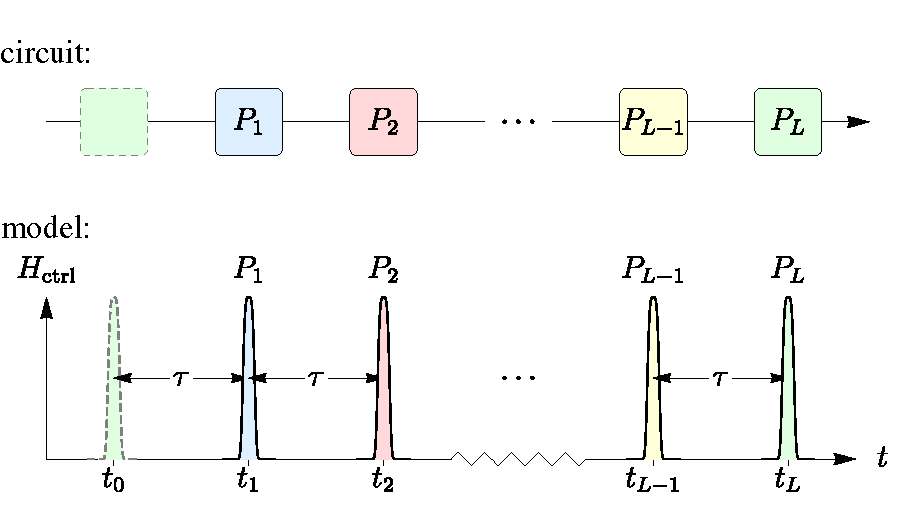
\includegraphics[width=1\linewidth]{pulse.pdf}
 \label{<label>}
\end{figure}

In the diagram, $Q_i$ is the computational gate ($=I$ for quantum memory) to be ``protected'' with dynamical decoupling; the dash represents the ``wait time'' between two gates; two gates without dash in between should be combined into a single gate.
Given its periodic structure, to study the effect of the DD sequence, 
we only need to focus on the time evolution of the unit cycle. 
% To study the effectiveness of DD, we make the stationary interaction assumption and  focus exclusively on the time evolution of this unit cycle.

All DD schemes share some fundamental similarities. First, the gates are always chosen from a specific group of transformations $P_i \in \sG,\  1\le i\le K$.
Second, all sequences must satisfy the constraint that they multiply to identity:
\begin{equation}\label{eq:fundamental-constraint}
    P_K P_{K-1} \cdots P_1 = I,
\end{equation}
so that we do not introduce additional transformations to the system.
On the other hand, different strategies could differ in 
the following aspects. 
\numcircled{1} The transformation group $\sG$. For single qubit, the most obvious choice is perhaps the Pauli group $\{I,X,Y,Z\}$. Some simple schemes such as the spin-echo \cite{Hahn1950} and the CPMG sequence \cite{Carr1954,Meiboom1958} use only the subgroup $\{I,Z\}$.  
\numcircled{2} The cycle length $K$ and the specific arrangement of the gates. 
\numcircled{3} The time at which the gates are applied. In particular, we have  constant gate-interval schemes, such as the periodic DD (PDD) \cite{viola1999dynamical} and the concatenated DD (CDD) \cite{khodjasteh2005fault}; and variable gate-interval schemes, such as the UDD \cite{uhrig2007keeping}, the nested UDD (NUDD) \cite{wang2011protection} and 
the quadratic DD (QDD) \cite{kuo2011quadratic}.
In this paper,  we focus specifically on the constant time-interval schemes with Pauli gates. The underlying physical model is a constant-frequency quantum circuit, whose operating frequency is limited by a finite switch-time  $\Dt>0$ between consecutive gates. 
A DD unit cycle of length $K$ is assumed to start from time $t=0$ and end at $t=K\Dt\equiv T$. 

Two potential sources of error associated with the DD procedure can be identified: the noise induced by interaction between the system the bath, which we aim to eliminate; and the error introduced by the imperfect DD gates.
Here we refer to the case where the second noise source is absent as the idealistic decoupling; and the model where both sources of noise are present as the noisy decoupling.



\section{Idealistic decoupling}
\subsection{Generic theory}
We model the noise associated with the free evolution by
CPTP maps. For the time evolution up to $\Dt$, we can find a Hamiltonian operator $H$ responsible for generating the unitary transformation between the system and bath,
\begin{equation}
    \Ufree(\Dt)= \upe^{-\upi \Dt H}\equiv\upe^{-\upi \Omega},
\end{equation}
where $\Omega=\Dt H$ is also referred to as the dimensionless Hamiltonian, and generates the free-evolution noise channel according to \Eqref{eq:output-rhos}.

Ideally, the DD gates $\{P_i\}$ can be modeled as perfect pulses applied at time instances $\{t_i = i \Dt,\ i=1,\ldots, K\}$. 
We make the assumption that the Hamiltonian remains constant within the duration of the DD cycle,
the time evolution operator for the cycle can be written as
\begin{equation}\label{eq:UDD-ideal}
    U_\sDD =P_K \upe^{-\upi \Omega}   \cdots P_2\upe^{-\upi \Omega} P_1\upe^{-\upi \Omega} = \upe^{-\upi \Odd},
\end{equation}
where we have assigned 
an effective Hamiltonian $\Odd$  for the whole cycle.

The constraint \Eqref{eq:fundamental-constraint} on the DD gates, together with the fact that all gates form a group, allow us to split each gate into a product of two hypothetical gates, $P_i = G_{i+1}^\dagger G_{i} \ (1 \le i \le K)$ with $G_1 = G_{K+1}= I$.
In light of this, specifying a sequence of DD gates $(P_1, \ldots ,P_K)$ is equivalent to specifying a sequence of gates $(G_2, \ldots ,G_K)$ without any constraint.
Substituting the splitting into \Eqref{eq:UDD-ideal} and taking the matrix logarithm, we get
\begin{equation}\label{eq:formal-Odd}
\Odd = \upi \log( 
\upe^{-\upi \Omega_K} \, \cdots \,\upe^{-\upi\Omega_2} \upe^{-\upi \Omega_1} ),
\end{equation}
where we define $\Omega_i \equiv G_i \Omega G_i^\dagger$.
The necessary convergence criteria is also assumed to ensure the existence of the matrix logarithm.

The \Eqref{eq:formal-Odd} gives the formal solution of the DD transformation on the noise dynamics, but in general cannot be analytically solved.
To proceed, one need to resort to 
approximation methods. This can be done by combining the matrix exponentials via the BCH formula, or by performing the Magnus expansion for time-dependent Hamiltonian.
Both approaches give the identical result by expressing the exponent as an infinite series,
\begin{equation}\label{eq:Oeff Magnus series}
   \Odd  = \sum_{m=1}^\infty \Odd\up{m},
\end{equation}
where the size of the $k$th term is of the order $\cO(\norm{\Omega}^k)$. Compared with the BCH formula approach, the Magnus expansion approach allows easier derivation for large $K$ and predicts a broader convergence bound.
From the theory of Magnus expansion \cite{blanes2009magnus}, a sufficient condition for  (\ref{eq:Oeff Magnus series}) to converge by absolute value is
\begin{equation}\label{dd:Magnus-abs-converge}
K\norm{\Omega }_\infty  < \xi=1.0868\cdots.
\end{equation}
The absolute-converge criterion is important for any finite truncation of the series (\ref{eq:Oeff Magnus series}) to make a reasonable approximation. 
In the following analysis, we assume such criterion is met.

Following the Magnus series formula, terms in \Eqref{eq:Oeff Magnus series} can be derived. In particular,  the first three terms can be calculated by the formula:
\begin{align}\label{eq:Magnus-12}
\Odd\up{1} = \sum_{i} \Omega_i,\quad
\Odd\up{2} =-\frac{\upi}{2} \sum_{i>j} [\Omega_i,\Omega_j], 
\end{align}
and 
\begin{align}\label{eq:Magnus-3rd}
\Odd\up{3} = -\frac{1}{6} \sum_{i\ge j\ge k}
\frac{ [\Omega_i,[\Omega_i,\Omega_k]]+[\Omega_k,[\Omega_j,\Omega_i]] }
{\mathrm{sym}({i,j,k})},
\end{align}
where the symmetry factor $\mathrm{sym}(i,j,k)$ is defined as the factorial product of the degeneracy of the indices, e.g., $\mathrm{sym}(3,2,2) =1!\times 2!=2$. In general, the $m$th order term can be written as a combination of nested commutators in $m$-fold copies of $\Omega_i$.
One can in principle apply the Magnus formula to obtain higher order terms,  but the expressions get complicated rapidly and effectively make direct derivations impractical. Instead, clever tricks that take advantage of the sequence structure need to be used.


According to \Eqref{eq:formal-Odd}, the DD protocol can be regarded as a transformation $\Omega \to \Odd$. Since the noise map $\cE$ is a function of $\Omega$ and $\rhoB$, the transformation on $\Omega$ takes the original quantum channel into a new 
one  $\cE\to\cE_\sDD$. 
As is argued in Sec.~\!\ref{sec:errph.vs.inf}, error phase is a convenient characterization of noise strength, we apply the two-component norm to the dimensionless Hamiltonian before and after DD, leading to 
\begin{align}
    \opnorm{\Omega} \equiv (\alpha,\beta) \quad \mathrm{and}\quad  \opnorm{\Odd} \equiv (\alpha_\sDD,\beta_\sDD).
\end{align}
The ``decoupling'' reference in the name of DD is understood in terms of the coupling part: i.e., the error phase of the new channel gets reduced through this transformation.
We say noise is suppressed if the ratio $\beta_\sDD/\beta<1$, and a lower ratio would indicate better noise suppression.


A widely used indicator to characterize the performance of DD schemes is the \emph{decoupling order}. A DD scheme is said to achieve $n$th-order decoupling  if the first $n$ terms in the series (\ref{eq:Oeff Magnus series}) have vanishing coupling part:
\begin{equation}\label{dd:nth-order-condition}
\Pcp(\Omega_{\sDD}\up{k}) =0,\ \text{for } 1\le k \le n.  
\end{equation}
The decoupling order is thus a single positive integer to grade different DD schemes. Greater decoupling order is usually linked with better noise suppression rate. 
This can be seen by evaluating the norm of the Magnus series projected on to the coupling part. For an $n$th-order decoupling sequence, we have
\begin{equation}\label{eq:nth-order-alternative}
\beta_\sDD 
=\norm[\Big]{\sum_{ k=n+1}^\infty \!\!\! \Pcp(\Omega_{\sDD}\up{k}) }
\simeq (\alpha,\beta)^{n+1},
\end{equation}
where we use the notation $(\alpha,\beta)^{n+1}$ to represent a polynomial that is $(n+1)$th order in $\alpha$ and $\beta$.
Provided that the Magnus series convergences absolutely, $\beta_\sDD$ is bounded by a power series in $\norm{\Omega}$ whose leading term is on the order of $n+1$.
Therefore \Eqref{eq:nth-order-alternative} provides an alternative characterization for the $n$th-order decoupling condition, which can be useful when directly calculating the first $n$ Magnus terms is unfeasible.




% Intuitively, DD is considered advantageous if the new channel is ``less noisy''. To make this idea more precise, we need some way to properly characterizing DD performance.

Meanwhile we may also employ the more sophisticated gauge of the channel distance and the channel infidelity to characterize DD performance. These indicators could accommodate the weakness in using error phase, particularly in cases with special symmetries.
For example, if one prepare the system in some decoherence-free subspace, applying the DD transformation $\Omega \to \Odd$ would break the initial symmetries and therefore increase the noise level according to the fidelity or distance measures. But this argument does not speak against the use of DD in general. 
The only promise of DD is to ``decouple'' the interaction Hamiltonian by reducing the magnitude of the coupling strength, and we shall consider the objective accomplished if DD serves such purpose.


In the following, we study two notable  DD  schemes with fixed pulsed interval and Pauli group pulses: periodic DD (PDD) \cite{viola1999dynamical} and concatenated DD (CDD) \cite{khodjasteh2007performance}. The PDD scheme can been seen as a special case of CDD. Our analysis showcases the steps to derive the fault-tolerance properties of DD and can be generalized to study other schemes.



\subsection{PDD}
For a single-qubit system coupled with a bath, we denote the free evolution Hamiltonian for time $\Dt$ as:
\begin{equation}\label{eq:omega-sq}
    \Omega = \Dt H = \sigma_0 \otimes B_0 + \sum_{i=1}^3 \sigma_i \otimes B_i,
\end{equation}
where 
$\{\sigma_i\}$ are the system space Pauli operators and
$\{B_i\}$ are the Hermitian bath operators with $\tr(B_0)=0$. The bath operators $B_i$ can be arbitrary dimensional, but are normalized such that  
\begin{equation}\label{eq:bathops-norm}
\opnorm{\Omega}
=
\begin{pmatrix}
\norm{B_0}\\
\norm[\Big]{\sum_{i=1}^3 \sigma_i \otimes B_i}
\end{pmatrix}\equiv\begin{pmatrix}
    \alpha\\
    \beta
    \end{pmatrix}.
\end{equation}

 

% For simplicity, we also represent $\Omega$ as a block vector $\vec{\Omega}$ in the Pauli  operator basis, whose $i$-th component equals to the bath operator $B_i$:
% \begin{equation}\label{dd:basis-vec}
% \renewcommand{\arraystretch}{1.5}
% \vec{\Omega}  \repr
% \begin{bmatrix}
%     B_0 \\\hline
%     B_1 \\
%     B_2 \\
%     B_3
% \end{bmatrix},
% \end{equation}
% where the horizontal line splits the pure bath part and the coupling part.


To reduce noise, we perform dynamical decoupling by periodically
applying the pulse cycle ``$-X-Z-X-Z$''.
The is also known as PDD scheme.
This cycle is sometimes referred to the universal decoupling sequence and it can suppress all types of noise on the qubit. 
Under the ideal-pulse assumption, the time evolution operator for the PDD cycle is:
\begin{equation}
Z \upe^{-\upi \Omega} X \upe^{-\upi \Omega} Z \upe^{-\upi \Omega} X \upe^{-\upi \Omega} 
\equiv \upe^{-\upi\Opdd},
\end{equation}
where an effective Hamiltonian $\Opdd$ is defined for the time evolution. The  transformation $\Omega\to\Opdd$ can be thought as an operator-valued function $\Opdd(\Omega)$.
Furthermore, since the resulting $\Opdd$ can be expressed as the Magnus series, 
each term in the series can be regarded as a function:
\begin{equation}\label{eq:PDD-update}
    \Opdd = \Opdd(\Omega) = \sum_{m=1}^\infty \Opdd\up{m}(\Omega).
\end{equation}
Applying the formula (\ref{eq:Magnus-12}), the first two terms in the series can by computed as:
\begin{align}\label{eq:PDD-magnus-1}
\Opdd\up{1}(\Omega) ={}  &\sigma_0 \otimes 4B_0 \\
\Opdd\up{2}(\Omega) ={} &\sigma_1 \otimes (-4\upi\,[B_0,B_1]) \notag \\
+\, &\sigma_2 \otimes (-2\upi\,[B_0,B_2] - 2\{B_1,B_3\}).\label{eq:PDD-magnus-2}
\end{align}
This explicitly verifies that PDD achieves first order decoupling as the coupling part vanishes for $\Opdd\up{1}$. 




\subsection{CDD}
Based upon PDD, a class of pulse schemes is proposed by Khodjasteh and Lidar \cite{khodjasteh2005fault} and named as CDD.
In this section, we present an independent analysis on CDD, with an emphasis  on the fault-tolerance (FT) perspective.
Previous paper on fault-tolerance also exist \cite{khodjasteh2007performance} with a focus on the quantum memory model. Our analysis is leant towards the quantum computation scenario. This results in different conclusions regarding the FT performance of CDD. Steps used in the derivation of CDD here also facilitate the development of the threshold criterion with noisy pulses.

To define the CDD scheme, we first denote the free time evolution operator as 
$U_{(0)}\equiv \upe^{-\upi \Omega}$, 
and the PDD time evolution operator as
$U_{(1)} \equiv \upe^{-\upi \Opdd}$. 
Higher level time evolution operators are defined recursively through the application of the PDD pulses on lower level maps:
\begin{equation}\label{eq:CDD-definition}
    U_{(k+1)} \equiv Z U_{(k)} X U_{(k)} Z U_{(k)} X U_{(k)}.
\end{equation}
Such recursion goes on until a predetermined maximum level is reached. For  concatenation level $n$, the resulting pulse sequence is denoted as  $\mathrm{CDD}_n$. We also associate an effective Hamiltonian for the time evolution operator at each level, 
$U_{(k)} \equiv \upe^{-\upi \Omega_{(k)}},\ k=1,\ldots, n$.
To construct the actual gate sequence for $\mathrm{CDD}_n$, we start with the recursive definition and then flatten out the nested levels by combining consecutive gates. This leads to the time evolution operator $U_{(n)}$ of the form (\ref{eq:UDD-ideal}) with $K=4^n$ gates to apply. 

Take $\mathrm{CDD}_2$ as an example, the eventual flattened gate sequence would be
``$-X-Z-X-Y-X-Z-X-I-X-Z-X-Y-X-Z-X-I$''. And in terms of the effective Hamiltonian, we have the following map:
\begin{equation*}
\begin{aligned}
\Omega_{(2)}=\upi \log(
&\upe^{-\upi \Omega }\upe^{-\upi X\Omega X}\upe^{-\upi Y\Omega Y}\upe^{-\upi Z\Omega Z}
\upe^{-\upi X\Omega X}\\
&\upe^{-\upi \Omega }\upe^{-\upi Z\Omega Z}\upe^{-\upi Y\Omega Y}
\upe^{-\upi Y\Omega Y}\upe^{-\upi Z\Omega Z}\upe^{-\upi \Omega }\\
&\upe^{-\upi X\Omega X}
\upe^{-\upi Z\Omega Z}\upe^{-\upi Y\Omega Y}\upe^{-\upi X\Omega X}\upe^{-\upi \Omega }).
\end{aligned}  
\end{equation*}
After applying \Eqref{eq:Magnus-12}, and \Eqref{eq:Magnus-3rd} to calculate the first three Magnus series, we find $\Omega_{(2)}\up{1} = \sigma_0 \otimes 16 B_0$, $\Omega_{(2)}\up{2} =0$, and $\Omega_{(2)}\up{3} \neq 0$ (for both  pure-bath part and coupling part). This shows that $\mathrm{CDD}_2$  achieves second order decoupling. 

It was suggested by the authors of CDD that the decoupling order for $\mathrm{CDD}_n$  is $n$ \cite{khodjasteh2005fault}. This statement is correct, but their proof is logically flawed. Given its importance, here we explain why the original proof is insufficient and  provide a rigorous proof for the decoupling order.


For the generic $\mathrm{CDD}_n$, it is infeasible to flatten out the gates and calculate the combined Magnus series directly. 
Instead it is easier to study the iteration map 
\begin{equation}\label{eq:CDD-update}
    \Omega_{(n)} = \Opdd(\Omega_{(n-1)}) = \sum_{m=1}^\infty \Opdd\up{m}(\Omega_{(n-1)}),
\end{equation}
where the update map $\Opdd$ is defined in \Eqref{eq:PDD-update}.
Backtracking the map from level $n$ to level $0$, we have
$\Omega_{(n)} = \Opdd\circ \cdots \circ \Opdd(\Omega)
\equiv(\Opdd)^n(\Omega)$.
In the end, the effective Hamiltonian $\Omega_{(n)}$ can be expanded as:
\begin{equation}\label{eq:CDD-magnus}
    \Omega_{(n)} =\sum_{m=1}^\infty \Omega_{(n)}\up{m}(\Omega),
\end{equation}
where $\Omega_{(n)}\up{m}$, with the size of  $\cO(\norm{\Omega}^m)$, is the $m$th order Magnus term in $\Omega$ . Notice that this series is different from the series in \Eqref{eq:CDD-update}, where
each $\Opdd^{(m)}$ generate the $m$th order Magnus term in $\Omega_{(k-1)}$.


To calculate the leading order Magnus term in $\Omega$, we do not directly solve $\Omega_{(n)}$ but instead constructing an estimator $\Ohat_{(n)}$ which is easier to solve. 
Formally we have an estimator-error pair $(\Ohat_{(n)},\delta\Omega_{(n)})$ such that
\begin{equation}\label{eq:est+err}
    \Omega_{(n)} = \Ohat_{(n)} + \delta\Omega_{(n)}.
\end{equation}
The estimator $\Ohat_{(n)}$  is faithful if it captures the leading order behavior of $\Omega_{(n)}$. This is defined separately for the pure-bath part and the coupling part, as they are of different orders.
In other words, a faithful estimator should contain the first nonzero pure-bath part and the first nonzero coupling part of the series (\ref{eq:CDD-magnus}).
An equivalent statement is that the error must be of higher order than the estimator. To quantify this statement, we take the two-component norm for both 
$\delta\Omega_{(n)}$ and $\Ohat_{(n)}$, and demanding
\begin{equation}
\opnorm{\delta\Omega_{(n)}}\equiv
\begin{pmatrix}
\delta\alpha_{(n)}\\
\delta\beta_{(n)}
\end{pmatrix}
\ll 
\opnorm{\Ohat_{(n)}}\equiv\begin{pmatrix}
\widehat\alpha_{(n)}\\
\widehat\beta_{(n)}
\end{pmatrix},
\end{equation}
where the comparison is implied for both components and should be understood by comparing the leading powers of the polynomials in $\alpha$ and $\beta$. 
In essence, a ``smaller'' polynomial should have a larger leading power and thus is of higher order smallness. 
We refer readers to Appendix~\ref{app:polynomials} for more rigorous descriptions on ordering polynomials by their leading powers.
Furthermore, after taking the two-component norm and applying triangular inequality for \Eqref{eq:est+err}, we find,
\begin{equation}
    \widehat\beta_{(n)}-\delta\beta_{(n)}\le  \beta_{(n)}\le \widehat\beta_{(n)}+\delta\beta_{(n)}.
\end{equation}
According to \Eqref{eq:nth-order-alternative}, the $n$th-order decoupling condition requires $\beta_{(n)}$ to be an $(n+1)$th order polynomial in $\alpha$ and $\beta$. It now suffices to show that \numcircled{1} $\widehat\beta_{(n)}$ is an $(n+1)$th order polynomial and \numcircled{2} the estimator is faithful.





The original CDD paper (Ref.\cite{khodjasteh2005fault}) constructed an estimator by keeping the first two Magnus terms for each iteration step. In
our notation:
\begin{equation}
    \Ohat_{(n)} \equiv (\Opdd\up{1} + \Opdd\up{2}) (\Ohat_{(n-1)}) = \big(\Opdd\up{1} + \Opdd\up{2}\big)^n (\Omega).
\end{equation}
With $\Opdd\up{1}, \Opdd\up{2}$ explicitly defined in \Eqref{eq:PDD-magnus-1} and \Eqref{eq:PDD-magnus-2}, and the starting point $\Ohat_{(0)}\equiv\Omega$,  the estimator can shown to be specified by the formula:
\begin{align}\label{eq:cdd-estimator}
\Ohat_{(n)} 
={} & \sigma_0 \otimes 4^n B_0 \notag \\
+\ & \sigma_1 \otimes (-\upi)^{n} 2^{n(n+1)} \ad_{B_0}^{n}(B_1)\\ 
+\ & \sigma_2 \otimes (-\upi)^{n} 2^{n^2} \ad_{B_0}^{n-\!1}( \,[B_0,B_2] - \upi \{B_1,B_3\} \,). \notag
\end{align} 
After taking the two-component norm of the estimator, we have,
\begin{equation}
\begin{pmatrix}
\widehat\alpha_{(n)}\\
\widehat\beta_{(n)}
\end{pmatrix}
\simeq
\begin{pmatrix}
\alpha\\
\alpha^{n} \beta +\alpha^{n-1} \beta^2
\end{pmatrix},
\end{equation}
where $\simeq$ represents equal the leading powers as described in Appendix~\ref{app:polynomials}. 
This verifies that $\widehat\beta_{(n)}$ is a an $(n+1)$th order polynomial.

To complete the theory, it now remains to show that $\Ohat_{(n)}$ is indeed faithful. For simplicity, we make the recognition $\alpha\simeq\beta\simeq\Dt$.
This change does not affect the criteria for $n$th order decoupling as the polynomial order is unchanged. To show $\delta\alpha_{(n)}$ and $\delta\beta_{(n)}$ are of higher order in $\tau_0$ compared to $\widehat\alpha_{(n)}$ and $\widehat\beta_{(n)}$, we claim that:
\begin{equation}\label{eq:cdd-error-bounds}
\begin{pmatrix}
\delta\alpha_{(n)}\\
\delta\beta_{(n)} 
\end{pmatrix}
\lesssim
\begin{pmatrix}
\Dt^3\\
\Dt^{n+2} 
\end{pmatrix}.
\end{equation}
We prove this assertion by mathematical induction.
At $n=1$,  i.e.\ the PDD sequence, the error comes solely from the Magnus series truncation.
Taking the two-component norm and applying triangular inequality:
\begin{equation}
\opnorm{\delta\Omega_{(1)}}\le\sum_{m=3}^\infty \opnorm{\Omega_{(1)}\up{m}}
\simeq \opnorm{\Omega_{(1)}\up{3}} \lesssim
\begin{pmatrix}
\Dt^3\\
\Dt^3
\end{pmatrix}.
\end{equation}
By definition, the higher level error term $\delta\Omega_{(n+1)}$ can be 
expressed with the lower level functions as:
\begin{multline}\label{eq:error update}
\delta\Omega_{(n+1)} 
=\Opdd(\Omega_{(n)})-(\Opdd\up{1}+\Opdd\up{2})(\Ohat_{(n)})\\
= \Opdd\up{1}(\delta\Omega_{(n)})+ \sum_{m=2}^\infty \Opdd\up{m}(\Omega_{(n)})-\Opdd\up{2}(\Ohat_{(n)}),
\end{multline} 
where we have used the fact that $\Opdd\up{1}$ is a linear map. Assuming  \Eqref{eq:cdd-error-bounds} holds for level $n$, we need to show $\opnorm{\delta\Omega_{(n+1)}}\lesssim(\Dt^3,\Dt^{n+3})$.
The argument in the original CDD paper by Khodjasteh and Lidar for truncating the Magnus series have only showed that the higher order Magnus term is smaller by proving
\begin{equation*}
    \opnorm{ \sum_{m=3}^\infty\Opdd\up{m}(\Ohat_{(n)}) } \ll \opnorm{\Ohat_{(n+1)}}.
\end{equation*}
If we take $\delta\Omega_{(n)}=0$, \Eqref{eq:error update} would identity the l.h.s.\  of above as $\opnorm{\delta \Omega_{n+1}}$, then this inequality would indeed indicate that the error term is of higher order.
However \Eqref{eq:error update} suggests that this argument is not sufficient: as
the estimate error $\delta\Omega_{(n+1)}$ comes not only  from the truncation error of the same level, but also accumulates from the lower level error $\delta\Omega_{(n)}$. 
To properly bound the size of the error term, we take the two-component norm on both sides of \Eqref{eq:error update}:
\begin{equation}
\begin{aligned}\label{eq:cdd-error-3terms}
\opnorm{\delta\Omega_{(n+1)} }
&\lesssim \opnorm{ \Opdd\up{1}(\delta\Omega_{(n)}) } + 
\opnorm{\Opdd\up{3}( \Omega_{(n)})} \\
&+ \opnorm{ \Opdd\up{2}(\Ohat_{(n)}+\delta\Omega_{(n)})-\Opdd\up{2}(\Ohat_{(n)})},
\end{aligned}    
\end{equation}
where the infinite sum of Magnus terms higher than third order is lead by the non-vanishing third order. 
We now examine the size of these terms.
The first term in (\ref{eq:cdd-error-3terms}) is easy,
\begin{equation*}
\opnorm{\Opdd\up{1}(\delta\Omega_{(n)})} = \begin{pmatrix}
4 \delta\alpha_{(n)} \\
0
\end{pmatrix}\simeq
\begin{pmatrix}
\Dt^3 \\
0
\end{pmatrix}.
\end{equation*}
To bound the size of the second term, we make two observations for the PDD Magnus series greater than the third order:
\begin{enumerate}
    \item At least one $B_{i\neq0}$ is involved in the coupling part.
    \item At least two $B_{i\neq 0}$ is involved in pure bath part.  
\end{enumerate}
% That is to say, for $\opnorm{X}=(\alpha,\beta)$, 
% the size of  the $m$th order Magnus term can be estimated by
% \begin{equation}
%     \opnorm{\Opdd\up{m}(X)} \lesssim \begin{pmatrix}
%         \beta^2 (\alpha+\beta)^{m-2} \\
%         \beta (\alpha+\beta)^{m-1}
%     \end{pmatrix}, \quad m\ge3.
% \end{equation}
Therefore, the second term can be bounded by
\begin{equation*}
\opnorm{\Opdd\up{3}(\Omega_{(n)})} 
\lesssim\begin{pmatrix}
\beta_{(n)}^2 (\alpha_{(n)}+\beta_{(n)}) \\
\beta_{(n)} (\alpha_{(n)}+\beta_{(n)})^2
\end{pmatrix}
\simeq \begin{pmatrix}
\Dt^{2n+2}\\
\Dt^{n+3}
\end{pmatrix},
\end{equation*}
where we have used $\alpha_{(n)}\lesssim\widehat\alpha_{(n)}$ and $\beta_{(n)}\lesssim\widehat\beta_{(n)}$ according to the induction hypothesis.
This can be alternatively shown by explicitly calculating the third order Magnus term using \Eqref{eq:Magnus-3rd}. 
To bound the third term in (\ref{eq:cdd-error-3terms}), we can calculate the difference $\Opdd\up{2}(\Ohat+\delta\Omega) - \Opdd\up{2}(\Ohat)$
using the expression for $\Opdd\up{2}$ from \Eqref{eq:PDD-magnus-2}.  In the end,
\begin{equation*}
\begin{split}
&\opnorm[\big]{\Opdd\up{2}(\Ohat+\delta\Omega) - \Opdd\up{2}(\Ohat)} 
\lesssim\begin{pmatrix}
    0\\
    \delta\alpha_{(n)}\delta\beta_{(n)}
\end{pmatrix}\\
&+\begin{pmatrix}
    0\\
    \widehat\beta_{(n)}\delta\alpha_{(n)} + \widehat\alpha_{(n)} \delta\beta_{(n)}
    +\widehat\beta_{(n)} \delta\beta_{(n)} 
\end{pmatrix}\simeq
\begin{pmatrix}
    0\\
    \Dt^{n+3}
\end{pmatrix}.
\end{split}
\end{equation*}
Since all three terms are bounded by $(\tau_0^3, \tau_0^{n+3})^\transpose$, so is their sum. This proves our assertion \Eqref{eq:cdd-error-bounds}. \qed

\smallskip

Having showed its faithfulness, we are now confident in using the estimator \Eqref{eq:CDD-magnus} to study the full $\Omega_{(n)}$ of $\mathrm{CDD}_n$. In particular, we have $\alpha_{(n)}\approx\widehat\alpha_{(n)}=4^n \alpha$ and
$\beta_{(n)}\approx\widehat{\beta}_{(n)}$.
Similar as the PDD case, we can derive a strict bound and an approximate bound. For the strict bound, we have
\begin{equation}\label{eq:cdd-errph-bound1}
\begin{aligned}
\widehat{\beta}_{(n)} &\le   2^{n(n+1)}\norm{\ad_{B_0}^{n}(B_1)} \\
&\quad + 2^{n^2} 
\norm{\ad_{B_0}^{n-\!1}([B_0,B_2] - \upi \{B_1,B_3\})}\\
&\le  2^{n(n+1)}\alpha^{n-1}\beta (2^n \alpha+ \alpha + \beta).
\end{aligned}
\end{equation}
From this upper bound,
we see that as the concatenation level goes up, $\widehat \beta_{(n)}$ would first decrease due to the small $\alpha$ value, but then start to increase 
due to the super-exponentially growing coefficient. This suggests the existence of a maximally allowed concatenation level, beyond which increasing the concatenation level would only introduce more noise. This can be seen explicitly from Fig.~\ref{fig:estimator-size}, where the relevant sizes of $\widehat \alpha_{(n)}$ and $\widehat \beta_{(n)}$ are plotted against the concatenation level in the logarithmic scale.
\begin{figure}[htbp]
    \centering
    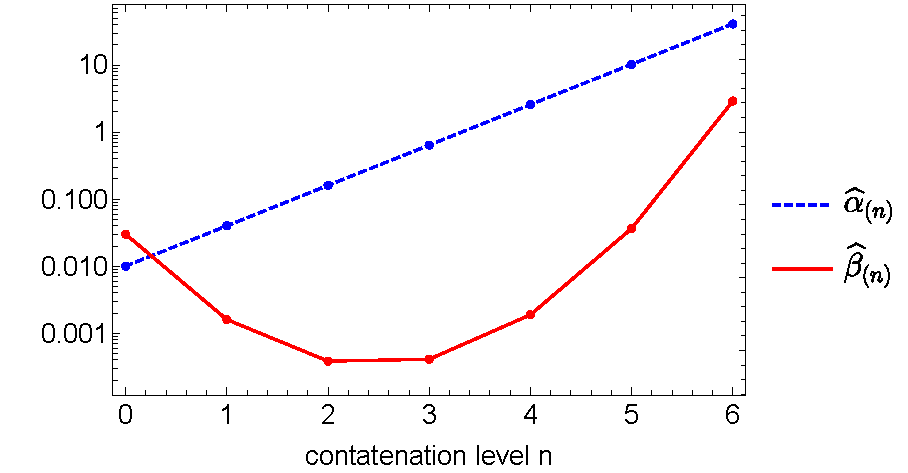
\includegraphics[width=0.9\linewidth]{cdd-estimator}
    \caption{The estimator size for $\widehat \alpha_n$ and the error phase $\widehat \beta_n$ as a function of concatenation level $n$. In the graph, the bare Hamiltonian is set to take on the value $\alpha=0.01$ and $\beta=0.01$.}
    \label{fig:estimator-size}
\end{figure}
For higher concatenation level to make sense, increasing concatenation level should decrease the error phase. To derive a sufficient condition for the maximal concatenation level, we compare the error phase upper bound in \Eqref{eq:cdd-errph-bound1} of the  $\mathrm{CDD}_n$ to that of the $\mathrm{CDD}_{n+1}$,
\begin{equation*}
\frac{2^{(n+1)(n+2)}\alpha^{n}\beta (2^{n+1} \alpha+ \alpha + \beta)}{2^{n(n+1)}\alpha^{n-1}\beta (2^n \alpha+ \alpha + \beta)} \le 4^{n+1}2\alpha.
\end{equation*}
The maximal level is reached when there is a contraction.
By requiring the r.h.s.\  to be smaller than 1, we obtain the bound for the maximal concatenation level:
\begin{equation}\label{eq:cdd-max-level}
n_{\max}\le -\log_4\alpha-\frac{3}{2}.
\end{equation}
The existence of a maximal concatenation level does not contradict with
the higher order decoupling achieved by higher level CDD. 
It simply means that the correspondence between higher decoupling order and better noise suppression is not always true. 
Generally, if the absolute converge criteria \Eqref{dd:Magnus-abs-converge}, is fulfilled, a higher $n$ means the leading order term is smaller. 
But if the DD scheme is designed such at the sequence length $K$ grows exponentially with $n$,
increasing $n$ will break the absolute convergence and the decoupling order is no longer a reasonable indicator. 



\section{Noisy Decoupling and Fault-Tolerance}

To determine whether DD should be implemented on a particular system,
one need to take on the fault tolerance perspective by weighing the costs and benefits of DD. If the benefits of doing DD outweigh the costs, DD should be encouraged; otherwise DD should be avoided. 

To begin with, it is important to 
distinguish whether the task is to preserve states in quantum memory, or to protect gates from noise in quantum computation. 
For quantum memory, the goal is to preserve quantum states for as long as possible. Whether implementing DD or not will not change the total evolution time. For quantum computation, on the other hand, the introduction of extra DD pulses dilate the time interval between computational gates.  Longer gate interval allows more time for noise to develop, potentially counteracting the benefit of DD.
Therefore despite the same transformation $\Omega\to \Omega_{\sDD}$ for both cases, the relevant transformation in terms of the time evolution operator, is $\upe^{-\upi K \Omega} \rightarrow\upe^{-\upi \Odd}$ for quantum memory and  $\upe^{-\upi \Omega} \rightarrow\upe^{-\upi \Odd}$ for quantum computation. 
In terms of the error phase, DD introduces the transformation: $\beta \to \beta_\sDD$.
For a DD sequence with cycle length $K$, we can formulate the  criteria for noise reduction in terms of error phase as
\begin{align*} 
\beta_\sDD&\le K\beta \quad &&\text{for quantum memory,}   \\
\beta_\sDD&\le \beta \quad &&\text{for quantum computation.}
\end{align*}
% The quantum memory case has a easier condition and has already been discussed in some past papers. 
In this the paper, we focus primarily on the quantum computation scenario.

The conditions for achieving noise suppression are already derived previously for the idealistic PDD and CDD case.
In general, we find that smaller $(\alpha,\beta)$ values would lead to to better noise suppression rate. Therefore the gates should be performed as frequently as possible. But this may leads to suboptimal outcomes in practice given the extra noise introduced by imperfect gate operations. To study the fault-tolerance of DD, we must account for the additional noise associated with the control gates.


\subsection{idealistic}

To determine when is PDD useful, we compare the error phase by solving $\beta_\mathsf{PDD}\le\beta$.
A precise solution is in general impossible as the full series (\ref{eq:PDD-update}) is unknown. We instead look for approximate solution using the leading order approximation and solve for 
\begin{equation}
    \beta_\mathsf{PDD}\approx \norm{\Opdd\up{2}(\Omega)}\le \beta
\end{equation}
To solve this inequality, we need 
to express the error phase in terms
of the bath operators.  We note the following inequalities:
\begin{align}\label{eq:errph-strict}
    \max_{i\in\{1,2,3\}} \norm{B_i}\le \norm[\Big]{\sum_{i=1}^3 \sigma_i \otimes B_i} \le \sum_{i=1}^3 \norm{B_i}.
\end{align}
The proof is given in Appendix~\ref{app:norm-ineq}. We use these bounds to derive a ``strict condition''. First, 
\begin{align}
\norm{\Opdd\up{2}(\Omega)} &\le
4\norm{[B_0,B_1]} +2\norm{\upi [B_0,B_2] +\{B_1,B_3\}} \notag \\
&\le 8 \alpha \norm{B_1} + 4 \alpha \norm{B_2} + 4\norm{B_1}\norm{B_3} \notag\\
&\le 12\alpha\beta +4\beta^2,
\end{align}
we then bound the last line by $\beta$ to arrive at: 
\begin{equation}\label{eq:pdd-region-strict}
    12\alpha + 4\beta \le 1.
\end{equation}

On the other hand, the inequalities (\ref{eq:errph-strict}) 
inspires use to use the following approximation for the error phase:
\begin{equation}\label{eq:errph-approx}
    \norm[\Big]{\sum_{i=1}^3 \sigma_i \otimes B_i} \approx \sqrt{\sum_{i=1}^3 \norm{B_i}^2}.
\end{equation}
Such approximation is valid up to a factor $\in[1/\sqrt{3},\sqrt{3}]$.
This approximation allows us to derive an ``approximate condition''. 
We estimate
\begin{align}\label{eq:beta2-pdd-estimate}
\beta_\mathsf{PDD}^2 & \approx
\norm{-4\upi  [B_0,B_1]}^2 +\norm{-2\upi  [B_0,B_2] - 2 \{B_1,B_3\}}^2 \notag \\
&\le (8\alpha \norm{B_1})^2 + (4\alpha\norm{B_2} + 4\norm{B_1}\norm{B_3})^2,
\end{align}
Defining $x_i\equiv\norm{B_i}/\beta$, then upper-bounding the r.h.s.\  by $\beta^2$ requires
\begin{equation}\label{eq:PDD-optimization}
\max_{\mathclap{x_1^2+x_2^2+x_3^2=1}} \  (2 \alpha x_1)^2 + (\alpha x_2 + \beta x_1 x_3)^2\le \frac{1}{16}.
\end{equation} 
Solution of this constrained optimization problem leads to:
\begin{equation}\label{eq:pdd-region}
\begin{aligned}
\Bigl(\frac{\beta}{\sqrt{3}}\le \alpha \le \frac{1}{8} \Bigr)
\ \mathrm{or}\ \Bigl(10 \alpha ^2+\frac{9 \alpha ^4}{\beta ^2}+\beta ^2\leq \frac{1}{4}\Bigr). 
\end{aligned}   
\end{equation}
This set of inequalities automatically implies (\ref{eq:pdd-region-strict}),
it gives a broader but less confident condition due to the approximation used
for the error phase.


The criteria (\ref{eq:pdd-region-strict}) and (\ref{eq:pdd-region}) each determines a region in the $(\alpha,\beta)$ parameter space where noise suppressing is achieved using the leading order Magnus term. 
But in order for the calculations to make sense, we have assumed that the Magnus series converge absolutely. According to (\ref{dd:Magnus-abs-converge}), the necessary condition here is $4 \norm{\Omega}_\infty   < \xi$.
Since $\norm{\Omega} \le \alpha +\beta$, we may use 
a more stringent convergence bound:
\begin{equation}\label{dd:PDD-magnus-abs}
    \alpha +\beta \le \frac{1}{4}.
\end{equation}

To examine the accuracy of the two theoretical bounds, we perform numeric tests as a verification. We first randomly generate  four $2\times 2$ Hermitian matrices for the bath operators satisfying the normalization condition in \Eqref{eq:bathops-norm}, then simulate the PDD protocol and use matrix logarithm to find the actual $\Opdd$ and error phase $\beta_\mathsf{PDD}$.  For each fixed $(\alpha,\beta)$ point, we numerically maximize the error phase reduction ratio $\beta_\mathsf{PDD}/\beta$ over 1000 random instances. The result is presented in \Figref{fig:pdd-region}, where a point in blue color represents a greater-than-one ratio and  yellow color represents smaller-than-one ratio. Thus the graph reflects the true noise suppressing condition by the continuous yellow-colored region.
We also plot the boundaries for the two theoretical noise suppression region from (\ref{eq:pdd-region-strict}) and (\ref{eq:pdd-region}), together with the absolute convergence region (\ref{dd:PDD-magnus-abs}) for comparison. 

\begin{figure}[ht!]
\centering
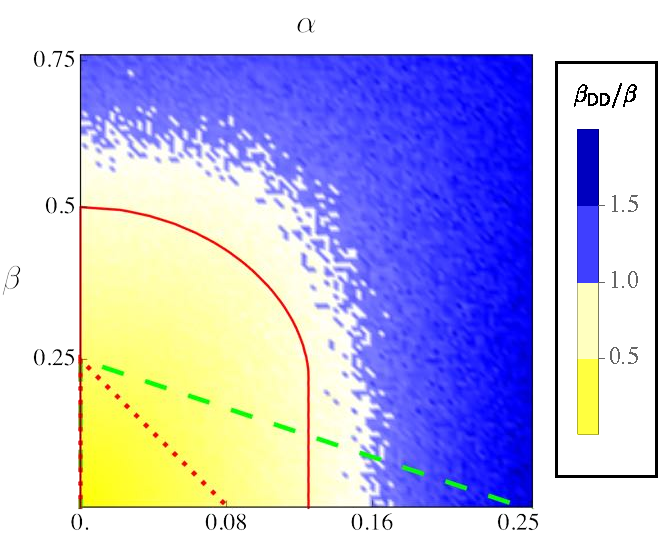
\includegraphics[width=0.8\linewidth]{pdd-ideal-region}
\caption{The noise reduction ratio $\beta_\sDD/\beta$ obtained through maximization over random bath operators plotted in the $(\alpha,\beta)$ parameter plane. In comparison, the theoretical boundaries for noise reduction are also plotted, with dotted red line for (\ref{eq:pdd-region-strict}) and solid red line for (\ref{eq:pdd-region}), also with the boundary for the absolute-convergence condition (\ref{dd:PDD-magnus-abs}) in dashed green line. Note the ranges for $\alpha$ and $\beta$ are chosen differently for better visual effect.}
\label{fig:pdd-region}
\end{figure}

As long as the two-component norm of the free evolution Hamiltonian falls in the yellow region on the lower-left corner, the idealist PDD scheme is guaranteed to work, in the sense of reducing the error phase. This reflects the fundamental ``small noise'' assumption of DD. From the numerical results, we learn that the bound by the ``strict condition'' from (\ref{eq:pdd-region-strict}) is too loose compared with the ``approximate condition'' (\ref{eq:pdd-region}), which works surprisingly well in reflecting the true boundary of the noise-reduction region. The faithfulness of the latter bound is particularly striking considering the points beyond the absolute-convergence boundary (above the green dotted line), where our derivation should be unreliable in principle. An explanation is that the absolute-convergence criteria (\ref{dd:PDD-magnus-abs}), sufficient but not necessary, is a loose one and the leading order Magnus series works well beyond the region predicted by this inequality. This piece of evidence boosts our confidence in using the leading order Magnus term as approximation in the following parts of this work. But for safety, the absolute convergence region will also be indicated. 


To best determine the noise suppressing condition for idealistic CDD, we follow  similar procedures as the PDD case by applying the error phase approximation \Eqref{eq:errph-approx},
\begin{align}
&\beta_{(n)}^2 \approx 2^{2n(n+1)}\norm{\ad_{B_0}^{n}(B_1)}^2 \notag \\
&\phantom{\beta_{n}^2 \approx} + 2^{2n^2} \norm{  \ad_{B_0}^{n}(B_2)+ \upi \ad_{B_0}^{n-1}(\{B_1,B_3\})}^2 \notag \\
&\le 4^{n(n+1)} \alpha^{2n-2} 
    \bigl( 4^n \alpha^{2} \norm{B_1}^2 +   ( \alpha \norm{B_2}+  \norm{B_1}\norm{B_3})^2 \bigr).
\end{align}
Defining $x_i\equiv\norm{B_i}/\beta$,
the noise reduction condition $\beta_{(n)}/\beta<1$ can be converted to the optimization problem:
\begin{equation}
\begin{split}
& \max_{\mathclap{ x_1^2+x_2^2+x_3^2=1 }} \; 4^n \alpha^{2} x_1^2 +  ( \alpha  x_2+ \beta x_1 x_3)^2\le 
\frac{1}{\alpha^{2n-2}  4^{n(n+1)}}.
\end{split}
\end{equation}
This inequality is satisfied when:
\begin{equation}
\begin{aligned}\label{eq:CDD-noise-removal}
& {\beta}/{\sqrt{4^n-1}} \le \alpha \le 1/2^{n+2} \ \\
\mathrm{or}\quad  &\Bigl(\dfrac{(4^n-1) \alpha^2 +\beta^2}{2\alpha\beta}\Bigr)^2+1  \le
\frac{1}{4^{n(n+1)}\alpha^{2n}}. 
\end{aligned}   
\end{equation}
This reduces to the PDD condition \Eqref{eq:pdd-region} when $n=1$ as one may easily check. Moreover, if the error phase $\beta\le\frac{1}{4} \sqrt{1-4^{-n}}\approx  1/4$, a realistic condition for small noise, it suffices to use the simplified cutoff for $\alpha$, 
\begin{equation}\label{eq:CDD-bound-simplified}
    \alpha \le \frac{1}{2^{n+2}}.
\end{equation}
Meanwhile we can establish the absolute convergence region of the Magnus series according to \Eqref{dd:Magnus-abs-converge}:
\begin{equation}\label{eq:CDD-converge}
    \alpha +\beta \le \frac{1}{4^n}.
\end{equation}

Now the sufficient condition promising a reduction of the error phase is for the two-component norm $(\alpha,\beta)$ of the initial Hamiltonian to fall in the overlapping region of \Eqref{eq:CDD-noise-removal} and \Eqref{eq:CDD-converge}. 
% These regions are plotted for concatenation level $n=1,2,3$ in Fig. \ref{fig:cdd-region} as a reference. 
% 
% \begin{figure}[ht!]
% \centering
% 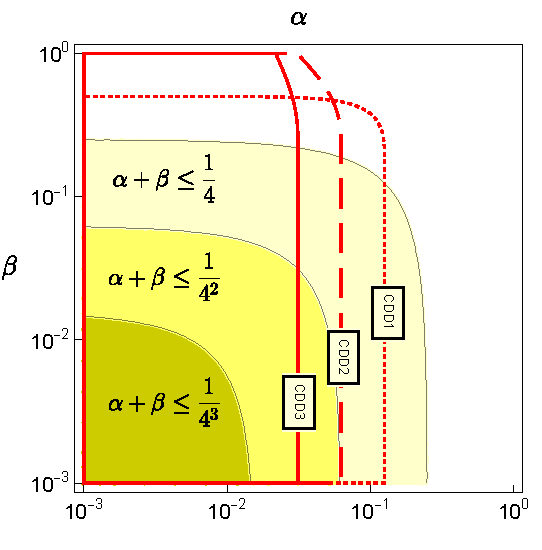
\includegraphics[width=0.8\linewidth]{cdd-region-1.pdf}
% \caption{The boundaries for the noise suppression region (red lines) and the absolute converge region (yellow shades) of the idealistic CDD compared for concatenation levels $n=1,2,3$. As the concatenation level goes up, the noise suppression and convergence region shrinks exponentially (noticing the logarithmic scales of the frame labels).} 
% \label{fig:cdd-region}
% \end{figure}
In general, the radius of the absolute convergence region gets exponentially smaller as the concatenation level goes up; and the convergence region completely falls in the region of noise removal for $n\ge 2$. This seems to suggest that the absolute convergence condition alone is enough.
But  numerical tests show that the Magnus series would typically convergence well beyond the region set by \Eqref{eq:CDD-converge},
the noise reduction condition \Eqref{eq:CDD-noise-removal} is more useful in 
representing the true noise suppressing region. Following a similar precedure as the PDD case, the noise reduction region is 
numerically scanned and compared with the predicted boundaries in \Figref{fig:cdd-scan} for level 2 and level 3 CDD.


\begin{figure}[ht]
\centering
% \begin{tabular}{cc}
% \includegraphics[height=0.48\linewidth]{cdd11-scan} &   \includegraphics[height=0.48\linewidth]{cdd12-scan} \\
% \includegraphics[height=0.46\linewidth]{cdd21-scan} &   \includegraphics[height=0.46\linewidth]{cdd22-scan} 
% \end{tabular}
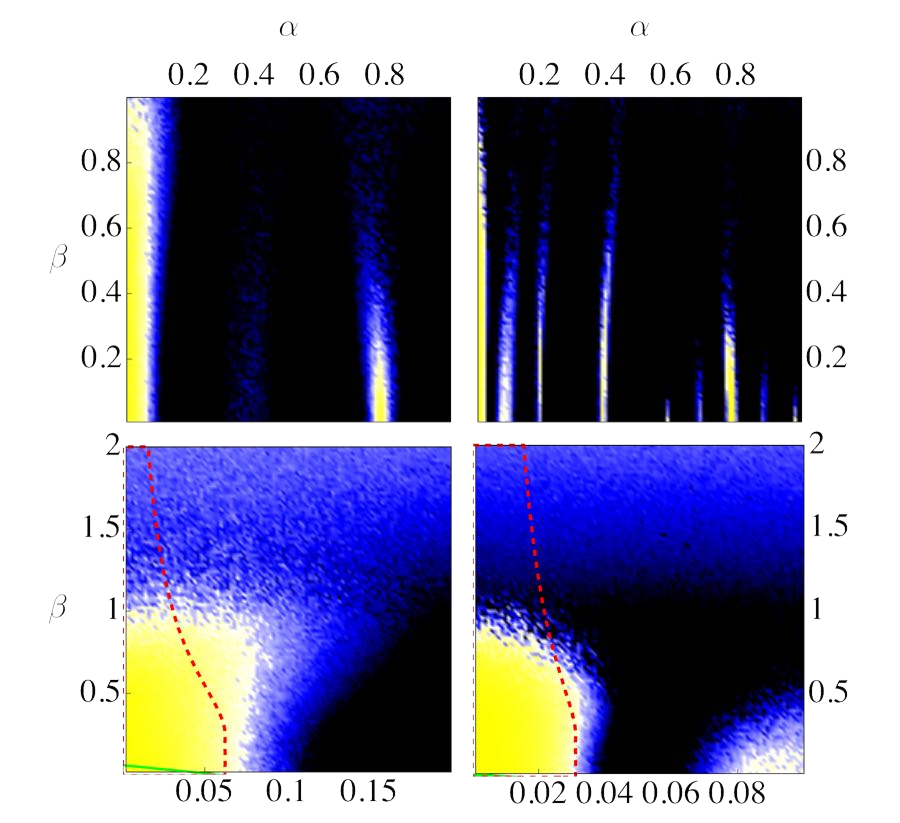
\includegraphics[width=\linewidth]{ICDD-grid}
\caption{The noise suppression region (in yellow) for CDD\textsubscript{2} (left) and CDD\textsubscript{3} (right) scanned over the $(\alpha,\beta)$ parametric plane.
Different ranges are used for the upper and lower graphs.
The red dotted lines indicated the theoretical suppression boundaries predicted by (\ref{eq:CDD-noise-removal}); the green solid line near the origin represents the absolute-convergence condition (\ref{eq:CDD-converge}).}
\label{fig:cdd-scan}
\end{figure}

From the noise suppressing region in \Figref{fig:cdd-scan}, we can conclude that the absolute convergence condition really fails to predict anything useful, especially for higher level CDD where the available region becomes too small---it is an indication of ``safeness'' but nowhere near the boundary. On the other hand, the bound (\ref{eq:CDD-noise-removal}) derived from the leading order Magnus approximation really prevails at reasonably small $\alpha$ and $\beta$ values, but fails when $\beta$ grows larger. In the end, it appears that the simplified bound (\ref{eq:CDD-bound-simplified}) works the best, as the free evolution noise should be small to start with. 
Another interesting observation is the yellow spikes at high $\alpha$ values shown in \Figref{fig:cdd-scan}. But such phenomenon is certainly beyond any prediction based on the Magnus series as it lays beyond the radius of converge Predicted by \Eqref{eq:CDD-converge}.

\subsection{Gate errors}

Generally, we can denote $\Pt_i =  P_i V_i$ as the noisy implementation of the gate $P_i$,
with $V_i\equiv P_i^\dagger \Pt_i$ representing the additional noise associated with the gate. 
If the noise is unitary, we can associate $V_i=\upe^{-\upi \Gamma_i}$, where $\Gamma_i$ is a Hermitian operator on $\cH_\rS$. 
For the CPTP noise case, we can find a unitary embedding by introducing an ancillary system $\cH_\rA$ (subscript ``A'' for ancilla), such that $V_i=\upe^{-\upi \Gamma_i}$ for some  Hermitian operator $\Gamma_i$ on the extended Hilbert space $\cH_\rS\otimes \cH_\rA$. These two scenarios can be unified if 
we allow $\dim(\cH_\rA)=1$.  
% Therefore we shall not distinguish between the two and only focus on the latter model for generality. 
The time evolution operator for a noisy DD cycle now becomes:
\begin{equation}\label{eq:UDD-noisy}
\begin{split}
\widetilde U_\sDD &\equiv \upe^{-\upi \widetilde\Omega_{\mathsf{DD}}} = \Pt_K \upe^{-\upi \Omega}   \cdots \Pt_2 \upe^{-\upi \Omega} \Pt_1 \upe^{-\upi \Omega}  \\
&=     P_K \upe^{-\upi \Gamma_K} \upe^{-\upi \Omega}   \cdots P_2 \upe^{-\upi \Gamma_2} \upe^{-\upi \Omega}  P_1 \upe^{-\upi \Gamma_1} \upe^{-\upi \Omega},
\end{split}
\end{equation}
where we have associated an effective Hamiltonian $\widetilde\Omega_{\mathsf{DD}}$ for the noisy DD cycle. For simplicity we make the assumption that $\cH_\rA$ and $\cH_\rB$ are disjoint Hilbert spaces. Then $\widetilde\Omega_{\mathsf{DD}}$ can be recognized as a Hermitian operator on the combined space $\cH_\rS\otimes \cH_\rA\otimes \cH_\rB$.
We also denotes its two-component norm by 
$\opnorm{\widetilde\Omega_{\mathsf{DD}}}= (\widetilde{\alpha}_\mathsf{DD},\widetilde{\beta}_\mathsf{DD})$. This can be done by viewing $\cH_\rA\otimes \cH_\rB$ as the new bath Hilbert space.
From its definition, we know that an extension of an irrelevant Hilbert space does not change the error phase.
So the change in the error phase results from the noise in the gates rather than the choice of ancilla space. 
We can now establish the noise threshold criteria for noisy DD gates by solving the error phase inequality $\widetilde{\beta}_\mathsf{DD}\le \beta$.
In the followings, We split our discussions according to the noise model considered.


 For gate-independent noise, 
 $\Pt_i = P_i V = P_i \upe^{-\upi \Gamma},\ \forall i$, a great simplification can be achieved in \Eqref{eq:UDD-noisy} by combining the gate-noise with the free-evolution noise into an effective free evolution map:
\begin{equation}\label{eq:noisy-merge}
    \Ut_\rf =  \upe^{-\upi \Gamma} \upe^{-\upi \Omega} \equiv 
    \upe^{-\upi \widetilde\Omega},
\end{equation}
where we have associate an effective Hamiltonian $\widetilde\Omega$ for the effective free evolution $\Ut_\rf$. To calculate the effective Hamiltonian $\widetilde\Omega_\sDD$ after such noisy DD,
we can simply replace the free evolution Hamiltonian $\Omega$ with $\widetilde{\Omega}$ and apply the same formula for calculating the idealistic DD.


It is thus imperative to understand how the gate error enters $\Omegat$.
Analytic expression for $\Omegat$ does not exist for non-commuting matrices. We can only express as it an infinite series by invoking the BCH formula,
\begin{equation*}
    \widetilde{\Omega} = \Gamma +  \Omega - \frac{\upi}{2} [\Gamma,\Omega]
    -\frac{1}{12}\bigl([\Gamma,[\Gamma,\Omega]]-[\Omega,[\Gamma,\Omega]]\bigr) + \cdots,
\end{equation*}
where higher order terms are nested commutators in $\Gamma$ and $\Omega$.
Just as $\Omega$ can be decomposed in to $\Omega_\rB + \Omega_\rSB$, we can apply a similar decomposition for $\Gamma$ as $\Gamma_\rA+\Gamma_\rSA$.
To characterize the gate error, we define its two-component norm by
\begin{equation}
    \norm{\Gamma_\rA} = \eta_0, \quad \norm{\Gamma_\rSA} = \eta.
\end{equation}
Per assumption, the ancilla and bath Hilbert spaces are disjoint. Therefore, $[\Omega_\rB,\Gamma] =[\Gamma_\rA,\Omega] =0 $. This indicates
that both $\Omega_\rB$ and $\Gamma_\rA$ would vanish in the BCH series  except for in the linear term, where they contribute to the 
pure bath part of $\Omegat$.
Defining $W \equiv \widetilde{\Omega} - \Gamma_\rA -  \Omega_\rB$, it then follows that $\Pcp(W)=\Pcp(\Omegat)$ and $\upe^{-\upi W} =  \upe^{-\upi \Gamma_\rSA} \upe^{-\upi \Omega_\rSB}$. As a result, we can bound the new error phase by
\begin{equation}\label{eq:beta-til-bound}
\begin{split}
    \widetilde{\beta}&\equiv\norm{\Pcp(\Omegat)} = \norm{\Pcp(W)}\le \norm{W}\\
    &= \norm{U_1 \Gamma_\rSA U_1^\dagger + U_2 \Omega_\rSB U_2^\dagger}
    \le \norm{\Gamma_\rSA} + \norm{\Omega_\rSB}\\
    &= \eta + \beta,
\end{split}    
\end{equation}
where we have applied the norm contraction property of the projection map $\Pcp$ on to the coupling space; the Thompson's formula \cite{Thompson1986} in line 2, which promises the existence of unitary matrices $U_1$ and $U_2$ such that 
$ W  = U_1 \Gamma_\rSA U_1^\dagger +   U_2 \Omega_\rSB U_2^\dagger$. 
On the other hand, as commutator of the traceless Pauli matrices remain traceless, $[\Gamma_\rSA,\Omega_\rSB]$ has no pure bath contribution. By expanding the series up to the third order, we can show
\begin{equation}\label{eq:alpha-til-bound}
    \widetilde\alpha \le \alpha + \eta_0 + \frac{1}{3} \eta \beta^2+\cO((\eta,\beta)^4).
\end{equation}
For small noise, it suffice to use the third order correction as an upper bound for $\alphat$.

These two bounds on $\alphat$ and $\betat$ can be used to derive the generic noise suppressing condition by the method of simple substitution.  Specifically, let's say that we have derived the error phase upper bound for idealist DD as a polynomial $f(\alpha,\beta)$ such that $\beta_\sDD \le f(\alpha,\beta)$ for all free evolution Hamiltonian specified by $(\alpha,\beta)$.  
% where $f(\alpha,\beta)$ is a polynomial of leading power $n+1$ for a DD scheme with decoupling order $n$.
This inequality would still apply for noisy DD 
given effective Hamiltonian specified by $(\widetilde\alpha,\widetilde\beta)$.
To compare with the free evolution case, we then upper-bound the maximal error phase after noisy DD by $f(\widetilde\alpha,\widetilde\beta) \le \beta$, now with the substitution $\alphat=\alpha+\eta_0+ \frac{1}{3}$ and 
$\betat =\beta + \eta$ as shown in \Eqref{eq:beta-til-bound} and \Eqref{eq:alpha-til-bound}.
This generic method of deriving threshold is conceptually simple and applies all DD schemes, but the resulting bound could be suboptimal.
Particularly when there is nested commutators in the expression of the DD estimator. To derive a better threshold, detailed analysis should be performed with respect to the specific DD scheme. 



\subsection{Gate independent noise}


Let us consider the noise suppressing condition for CDD 
under the gate-independent unitary noise model, where an over-rotation error is associated with all gates, $\Pt_i = P_i \upe^{-\upi \vec{\sigma} \cdot\vec{\theta}}$, where $\vec{\theta} = (\theta_1,\theta_2, \theta_3)^\transpose$.
There is no pure bath part here as it only contributes to a global phase, the error phase is given by the rotation angle $\norm{\vec{\theta}}\equiv\theta$.
Such type of noise could happen, for example, if their is a systematic calibration error in the system.

Let us expand the write the effective free evolution Hamiltonian from \Eqref{eq:noisy-merge} as:
\begin{equation}\label{eq:eff-free-part}
\begin{aligned}
    \widetilde{\Omega} &= \vec\sigma \cdot \vec \theta + \Omega'=  \sigma_0 \otimes B_0' + \sum_{i=1}^3 \sigma_i \otimes (\theta_i + B_i' ).  
\end{aligned}
\end{equation}
Up to second order in the BCH series, we have $B_0'\approx B_0$ and 
$B_i'\approx B_i + \sum_{jk} \epsilon_{ijk} \theta_j B_k,\ i=1,2,3$. 
Up to first order smallness in $\theta$, the expression for $(B_1',B_2',B_3')$ can obtained by rotating the vector $(B_1,B_2,B_3)$ with respect to the $\vec \theta$-axis.
On the other hand,  we know from its definition that the error phase is the invariant with respect to a basis change of the system, which acts as a 3D rotation on the vector $(B_1,B_2,B_3)$.
As a result, the error phase of $\Omega'$ remains identical to $\beta$ up to the second order in $\theta$. To conclude, the two-component norm of $\Omega'$ can be estimate by
\begin{equation}\label{eq:eff-Hami-tcp}
    \opnorm{\Omega'} = \begin{pmatrix}
        \alphat \\
        \beta'
    \end{pmatrix}
    \le 
    \begin{pmatrix}
        \alpha + \frac{1}{3}\theta\beta^2  \\
        \beta + \theta^2 \beta
    \end{pmatrix}.
\end{equation}
Assuming the noise to be small, we may only use the leading order 
approximation, knowing that it is accurate to the second order. 

We now calculate the noise suppression condition for $\mathrm{CDD}_n$, with PDD recognized as the special case of $n=1$. From the formula for the $\mathrm{CDD}_n$ estimator in \Eqref{eq:cdd-estimator} and the
 free evolution Hamiltonian $\Omegat$ in \Eqref{eq:eff-free-part}, we can estimate the coupling part of $\Omegat_{(n)}$ as 
\begin{align}
&\Pcp(\Omega_{(n)})
\approx \sigma_1 \otimes (-\upi)^{n} 2^{n(n+1)} \ad_{B'_0}^{n}(B'_1)\\ 
&\ + \sigma_2 \otimes (-\upi)^{n} 2^{n^2}\!\!\!\ad_{B'_0}^{n-\!1}\!\bigl(\,[B'_0,B'_2] - \upi \{B'_1+\theta_1,B_3'+\theta_3\}\bigr),\notag
\end{align} 
where all numbers $\theta_i$ in the commutators have been eliminated. We proceed to estimate the error phase upper-bound using the approximation formula \Eqref{eq:errph-approx} and applying triangular inequality for operator norm:
\begin{equation}
\begin{aligned}
&\beta^2_{(n)} 
% \approx \norm{2^{n(n+1)}\!\ad_{B'_0}^{n}(B'_1)}^2\\
% &\qquad + \norm{2^{n^2}\!\!\!\ad_{B'_0}^{n-1}\bigl(\,[B'_0,B'_2] - \upi \{B'_1+\theta_1,B_3'+\theta_3\}\bigr)}^2\\
\le 2^{2n(n+1)} \norm{B_0'}^{2n-2} \Bigl\{ (2^n  \norm{B_0'} \norm{B_1'})^2  \\
&\qquad + \bigl(\norm{B_0'} \norm{B_2'} +(\theta_1+\norm{B_1'})(\theta_3+\norm{ B_3'}) \bigr)^2 \Bigr\}.
\end{aligned}
\end{equation}
Upper-bounding the r.h.s.\ by $\beta^2$, we eventually arrive at the optimization problem:
\begin{align}\label{eq:ncdd-opt}
\mathop{\max_{x_i, y_i}}_{\mathclap{\norm{\vb x}=\norm{\vb y}=1}} \ 
& (2^n\alphat x_1)^2 + \Bigl(\alphat x_2 + 
\frac{(\theta y_1+\beta x_1)(\theta y_3+ \beta x_3)}{\beta}\Bigr)^2\notag\\
 &  \le \frac{1}{2^{2n(n+1)}\alphat^{2n-2}},
\end{align}
where we have recognized $\norm{B_0'}\le \alpha + \beta^2 \theta/3 \equiv \alphat$ and defined $x_i\equiv\norm{B_i'}/\beta$, $y_i\equiv\theta_i/\theta$.
The normalization constraint for $\vb x$ is set to $\norm{\vb x} = 1$ in stead of the original $\norm{\vb x} = \beta'/\beta$. According to \Eqref{eq:eff-Hami-tcp}, the deviation for this smaller norm is on the order of $\cO(\theta^2)$ which can be safely ignored as higher order smallness.

The analytical solution to this problem is not known to us, but we can instead solve a slightly weaker condition given all parameters are reasonably small. Next we bound the term involving $\vb y$ by
\begin{equation*}
    (\theta y_1+\beta x_1)(\theta y_3+ \beta x_3) \le \frac{1}{2} \theta^2 
    + \sqrt{x_1^2+x_3^2} \theta\beta + \beta^2 x_1 x_3,  
\end{equation*}
which can be shown by expanding the bracket and maximizing the coefficients individually. We also realize that the maximization should be achieved at around $x_2=0$ to take advantage of either a large $\alphat$ or a large $\betat$. This leads to the slightly weaker maximization problem:
\begin{align}\label{eq:ncdd-opt-weaker}
\max_{\mathclap{x_1^2+x_3^2=1}}\ 
& (2^n\alphat x_1)^2 + (\frac{\theta^2}{2\beta}+\theta +\beta x_1 x_3)^2\le \frac{1}{4^{n(n+1)}\alphat^{2n-2}},
\end{align}
whose solution can be now be found analytically, albeit complicated.
Now given a specific $\theta$ value, this inequality would determine a continuous region in the $(\alpha,\beta)$-plane where noise suppression is possible.  On the other hand, for a particular pair of $(\alpha,\beta)$ values, this inequality would determine a maximally allowed $\theta$.

Let us first focus on PDD.
In \Figref{fig:npdd-reg-tho},
We illustrate the noise suppression regions obtained from (\ref{eq:ncdd-opt-weaker}) for PDD with increasing levels of noise strength $\theta$.
This figure also intuitively demonstrates how the maximally allowed $\theta_{\mathrm{max}}(\alpha,\beta)$ depends on the parameters $(\alpha,\beta)$. 
In general, a smaller $\alpha$ value leads to a larger $\theta_{\mathrm{max}}$.  An optimal spot in the phase plane which is able to tolerant most error can be found at around near the $\alpha$-axis. 

\begin{figure}[htbp]
\centering
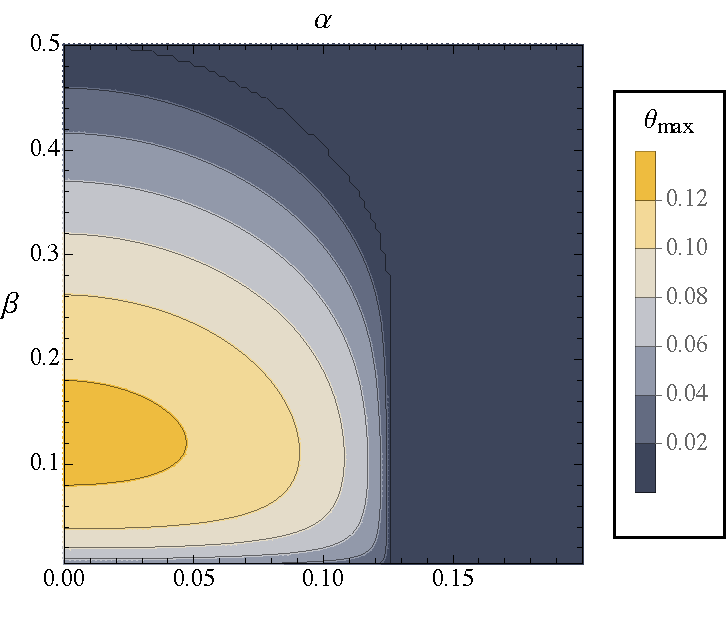
\includegraphics[width=0.8\linewidth]{npdd-region-thmax}
\caption{The noise suppressing region for noisy PDD with varying levels of noise $\theta$. Also can be understood as the contour plot of the maximally tolerable noise level $\theta_{\max}$.}
\label{fig:npdd-reg-tho}
\end{figure}

Another observation from \Figref{fig:npdd-reg-tho} is that the lower-left corner around the origin gradually leaves the noise suppressing region as the gates get noisier. This is because the noise associated with free evolution is small compared with the noise in the gates ($\beta\ll \theta$), so that the cost of noisy DD overwhelms its benefit. Thus this regime of is important for the purpose of deriving the gate error threshold.  
For $\beta\ll \theta$, the second parenthesis in \Eqref{eq:ncdd-opt-weaker} will dominate due to the small denominator. With the same logic, this approximation also applies to the regime where $\alphat \ll\beta$. In those cases, the optimization can then be approximately achieved by only considering maximizing the second term. This is achieved when 
$x_1=x_3=1/\sqrt{2}$ independent of the values of $\theta$ and $\beta$. Substituting this solution back to \Eqref{eq:ncdd-opt-weaker}, then we can predict the following simplified bound for PDD:
\begin{equation}\label{eq:npdd-bound-simple}
2\alphat^2 + \frac{(\theta+\beta)^4}{4\beta^2}\le \frac{1}{16},
\end{equation}
From this relation we can solve for $\theta$ in terms of $\alpha$ and $\beta$. After keeping the leading order terms, we arrive at the noise threshold for the rotation angle:
\begin{equation}\label{eq:npdd-err-thres}
    \theta \le (1-32 \alpha ^2)^{\frac{1}{4}} \sqrt{\frac{\beta}{2} }-\beta
    \quad \lesssim \sqrt{\frac{\beta}{2}}.
\end{equation}
It states that for the regime where the the free evolution noise is small, gate noise should at most be on the order of the square root of the free evolution noise for PDD to be considered worthwhile. 
Further more, from this inequality, it is clear that the maximally allowed $\theta$ is a monotonically decreasing function in $\alpha$. The globally maximally allowed $\theta$ can be found at $\alpha=0$, $\beta=1/8$ with
$\theta_\mathrm{max}= 1/8$.


\begin{figure}[htbp]
    \centering
        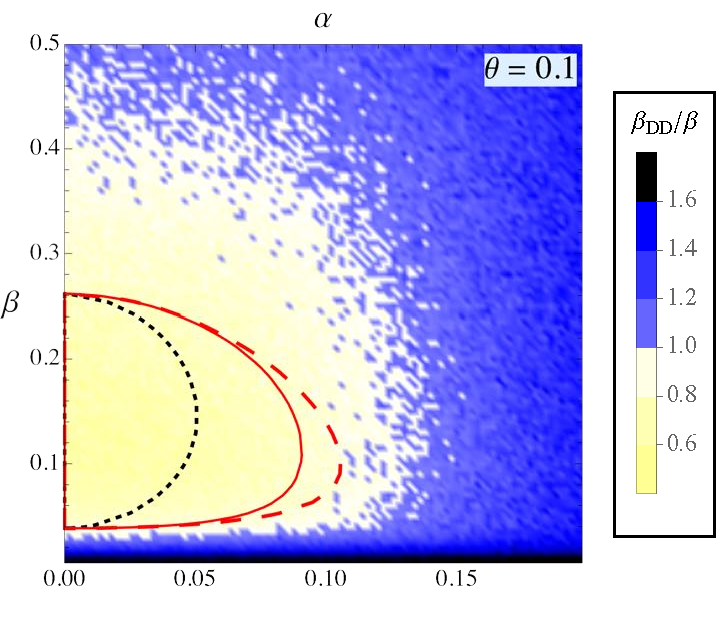
\includegraphics[width=0.8\linewidth]{npdd-region-num}
        \caption{The maximal $\beta_\sDD/\beta$ ratio obtained from numerical simulations for noisy PDD with $\theta=0.1$. Boundaries of the theoretic noise suppressing regions are marked for comparison: red solid line indicates result from optimization \Eqref{eq:ncdd-opt}, black dotted line stands for the generic boundary after simple substitution, and the red dashed line represents the approximate condition \Eqref{eq:npdd-bound-simple}.}
    \label{fig:npdd-reg-num}
    \end{figure}

To examine the validity of our results, we numerically simulate PDD with fixed unitary error at $\theta=0.1$. The simulation is performed in the similar manner as the ideal PDD case except with the additional errors. The data is presented in in \Figref{fig:npdd-reg-num},  together with the theoretical boundary 
predicted predicted by \Eqref{eq:ncdd-opt-weaker} marked in red solid line.
For comparison, the noise suppression bound from simple substitute of the ideal PDD condition with $\alpha\to\alphat$ and $\beta\to\betat$ is plotted in dashed black line; and the simplified bound  \Eqref{eq:npdd-bound-simple} is also plotted as dashed red line. 
We see that the three boundaries coincides at $\alpha=0$ while extending  differently into the parameter plane. The simple substitution strategy produces the smallest region. The optimized boundary from \Eqref{eq:ncdd-opt-weaker} gives a better result after taking into account of the commutator terms.   The approximate condition \Eqref{eq:npdd-bound-simple} works well in capturing the $\alpha\ll\theta$ behavior, but is already violated by numerical evidences from 
\Figref{fig:npdd-reg-num} for larger $\alpha$, as indicated by the blue dots within its boundary. Another observation from \Figref{fig:npdd-reg-num} is the relative insensitivity of the $\alpha$ value with respect to the noise suppression region, as indicated by the bottom boundary which is almost parallel to the horizontal axis. This insensitivity is also reflected in the 
error threshold condition \Eqref{eq:npdd-err-thres}.




As is the case for PDD, the trail solution $x_1=x_3=1/\sqrt{2}$ for \Eqref{eq:ncdd-opt-weaker} still gives a
decedent approximate solution for higher level CDD. 
After substitution, we have:
\begin{equation}\label{eq:ncdd-bound-simple}
2^{2n-1} \alphat^2 + \frac{(\theta+\beta)^4}{4\beta^2}\le \frac{1}{4^{n(n+1)}\alphat^{2n-2}},
\end{equation}
This inequality establishes the region where the error phase is reduced by CDD according to the leading order Magnus expansion. 
In \Figref{fig:ncdd-reg-thoery}, we plot the noise removal region determined by \Eqref{eq:ncdd-bound-simple} for $\mathrm{CDD}_2$ and $\mathrm{CDD}_3$ with different levels of noise $\theta$. Instead of plotting the entire phase space, we focus on the regime where $\alpha$ and $\beta$ are small, as defined by \Eqref{eq:CDD-bound-simplified}, so that our approximate condition is accurate.

\begin{figure}[htbp]
    \centering
    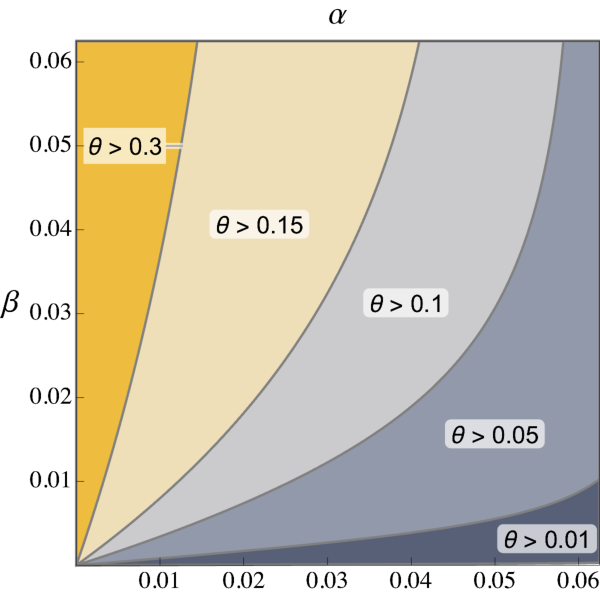
\includegraphics[width=0.45\linewidth]{ncdd2-region-thmax}\quad
    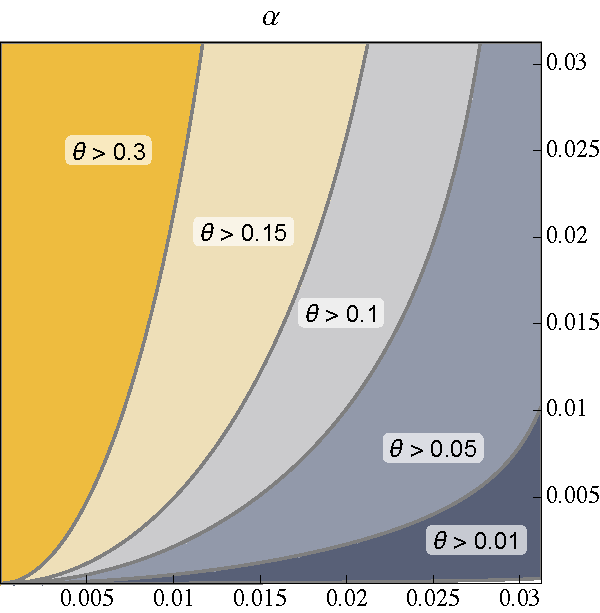
\includegraphics[width=0.45\linewidth]{ncdd3-region-thmax}
    \caption{The noise removal region of $\mathrm{CDD_2}$ (left) and $\mathrm{CDD_3}$ (right) for different levels of noise strength specified by $\theta$.
    Notice the ranges for $\alpha$ and $\beta$ are different for different concatenation levels. }
    \label{fig:ncdd-reg-thoery}
\end{figure}

Some differences can be seen by comparing \Figref{fig:npdd-reg-tho} and \Figref{fig:ncdd-reg-thoery}. In the PDD case, the noise reduction region quickly shrinks to a point as $\theta$ increases. But this is not the case for higher level CDD, where the region is pushed closer and closer to the $\alpha=0$ boundary.
Also as opposed to the PDD, there is no globally maximal $\theta_{\max}$ predicted from the noise suppressing condition \Eqref{eq:ncdd-bound-simple}.
This difference is most obvious by considering the $\alpha=0$ limit. According to \Eqref{eq:ncdd-bound-simple}, the r.h.s. blows up for $n\ge2$, implying very large noise can be tolerated.  
The counter-intuitive prediction of noise tolerance is clearly incorrect.
The fault stems from failure in approximating the Magnus seres by its leading order term. In \Eqref{eq:cdd-estimator} for the leading order term of the CDD effective Hamiltonian, all coupling part bath operators are expressed as nested commutators with $B_0$ for $n\ge2$. A vanishing $B_0$ therefore implies the diminish of the entire coupling part, leaving the next order term to be ``leading''. This argument also applies when $B_0\ne0$: while the error phase of the leading order term is $\cO(\alpha^n \beta)$, the next order term contains component on the order of $\beta^{n+2}$. Now that if $\alpha\ll \beta$, there is no way to be sure that $\alpha^n\beta \gg \beta^{n+2}$, which suggests that the higher order term could turn out to be larger than the estimator. Therefore, to correctly estimate the error phase of CDD and derive the noise threshold, we need to assume that $\alpha\neq 0$ and that $\alpha$ and $\beta$ are on the same order of smallness. 

We now assume that $\alpha$ and $\beta$ are of similar size. Then the approximation $\alphat \approx \alpha$ can be made.
From \Eqref{eq:ncdd-bound-simple}, we can solve for $\theta$ and keep the leading order terms in $\beta$. The following threshold can be obtained:
\begin{equation}\label{eq:cdd-threshold}
\theta\le  \left( (2^{n+2} \alpha)^{2(1-n)}-\tfrac{1}{2}(2^{n+2} \alpha)^2\right)^{\frac{1}{4}} \sqrt{\frac{\beta}{2}}-\beta.
\end{equation}
Supposing that ideal $\mathrm{CDD}_n$ is allowed, we can recognize the cutoff $(2^{n+2} \alpha) \le 1$  from \Eqref{eq:CDD-bound-simplified}. Since the coefficient before $\sqrt{\beta/2}$ is a monotonically decreasing function in $(2^{n+2} \alpha)$, which attains the minimal value at the cutoff. We can express the threshold in terms of the error phase alone:
\begin{equation}\label{eq:cdd-threshold-erph}
\theta\le  (1/8)^{\frac{1}{4}} \sqrt{\beta}-\beta.
\end{equation}
This threshold shows that for CDD the gate noise level should still be bounded by the square root of the free evolution noise level. This is consistent with our finding for the PDD case. One the other hand, for fixed free evolution Hamiltonian (therefore fixed $\alpha,\beta$), different CDD concatenation levels could turn out to have different noise thresholds due to the leading coefficient in \Eqref{eq:cdd-threshold} as a function of $n$. 
It turns out that there exists an optimal concatenation level in terms of the noise threshold. Let us say that $\alpha\approx 1/2^{N+2}$, $N\ge2$, so that the maximal 
allowed concatenation level is $N$. Substituting back to \Eqref{eq:cdd-threshold} and focusing on the term within the parenthesis, the following approximation can be made:
\begin{equation*}
    2^{2(n-N)(1-n)} - \tfrac{1}{2}2^{2(n-N)} \approx 2^{2(N-n)(n-1)}, \ 1\le n\le N.
\end{equation*} 
After maximizing the exponent, we find the optimal concatenation level is at 
$(N+1)/2$. This calculation suggests that increasing the concatenation level to the maximal allowed level may not be a good idea with noisy gates.  
Knowing the $\alpha$ value, it is possible to perform optimization on the coefficient to obtain the best concatenation level. Otherwise, one is advised to follow the generic threshold \Eqref{eq:cdd-threshold-erph}.

% To bound the error phase, we again apply the approximation \Eqref{eq:errph-approx} and the approximation for $\opnorm{\Omegat'}$, leading to 
% \begin{equation}
% \betat_\mathsf{PDD}^2 
% \le (8\alpha \norm{B_1'})^2 + (4\alpha\norm{B_2'} + 4\norm{\theta_1+B_1'}\cdot\norm{\theta_3+B_3'})^2.
% \end{equation}
% After defining $x_i\equiv\norm{B_i'}/\beta$ and $y_i\equiv\theta_i/\theta$ and bounding the r.h.s.\  by $\beta^2$, we arrive at the optimization problem:
% \begin{equation}\label{eq:npdd-opt}
% \max_{\mathclap{\stackrel{\norm{\vb x}=1}{\norm{\vb y}=1} }}\ 
% (2\alpha x_1)^2 + \Bigl(\alpha x_2 
% + \frac{(\theta y_1+\beta x_1)(\theta y_3+ \beta x_3)}{\beta}\Bigr)^2
% \le \frac{1}{16}.
% \end{equation} 
% \begin{equation}\label{eq:npdd-opt}
% \max_{\mathclap{\norm{\vb x}=1 }}\ 
% (2\alpha x_1)^2 + \Bigl(\alpha x_2 
% + \frac{\theta^2}{2\beta} + \theta\sqrt{x_1^2+x_3^2} + \beta x_1 x_3\Bigr)^2
% \le \frac{1}{16}.
% \end{equation} 

\subsection{gate-dependent noise}
Let us consider the case where noise is dependent on the gate. 

For PDD and CDD, as the sequence is composed of only the elementary $X$ and $Z$ gates, we assume that the noisy implementation of these gates are
\begin{equation}\label{eq:gatedep-noise}
\widetilde{X} = X \upe^{-\upi \Gamma'},
\quad \widetilde{Z} = Z \upe^{-\upi \Gamma''}.
\end{equation}
With these noisy gates substituted, the PDD time evolution map can be written as
\begin{equation}
\begin{split}
\upe^{-\upi \widetilde{\Omega}_\sP} &= Z \upe^{-\upi \Omega''}   X \upe^{-\upi \Omega'} Z \upe^{-\upi \Omega''} X \upe^{-\upi \Omega'}  \\
& = \upe^{-\upi Z\Omega''Z} \upe^{-\upi Y\Omega'Y} \upe^{-\upi X\Omega''X} \upe^{-\upi \Omega'},
\end{split}
\end{equation}
where we have defined 
\begin{equation}\label{eq:Omega-gatedep}
\upe^{-\upi \Omega'}\equiv \upe^{-\upi \Gamma'}\upe^{-\upi \Omega},\quad 
\upe^{-\upi \Omega''}\equiv \upe^{-\upi \Gamma''}\upe^{-\upi \Omega}.
\end{equation}
We can now apply the Magnus formula \Eqref{eq:Magnus-12} to solve for the PDD effective Hamiltonian 
$\widetilde{\Omega}_\sP$. 
Supposing that $\Omega' = \sum_i \sigma_i \otimes B'_i$ and 
$\Omega'' = \sum_i \sigma_i \otimes B''_i$ , the first two Magnus terms are 
now
\begin{align}\label{eq:PDD-gatedep-Mag1}
&\widetilde{\Omega}_\sP^{(1)} 
= \sigma_0 \otimes 2(B'_0 + B''_0) + \sigma_2 \otimes 2(B_2'-B_2'') \\[1ex]
&\widetilde{\Omega}_\sP^{(2)} = \notag
\sigma_0 \otimes \upi\,([B'_0,B''_0]+\![B'_1,B''_1]-\![B'_2,B''_2]-\![B'_3,B''_3]) \\[0.5ex]
&\! + \sigma_1 \otimes 
(-\upi\,[B_0'{+}B_0'',B_1'{+}B_1'']+\{B_2'{-}B_2'', B_3'{-}B_3''\}) \notag \\[0.5ex]
 &\!+ \sigma_2 \otimes 
(-\upi\,[B_0',B_2'']\!-\upi\,[B_0'',B_2'] -\! \{B_1',B_3''\}
 -\!\{B_1'',B_3'\} ) \notag\\[0.5ex]
 &\!+\sigma_3 \otimes 
(\upi\,[B_0'{+}B_0'',B_3''{-}B_3'] + \{B_1'{+}B_1'',B_2''{-}B_2'\}).
\label{eq:PDD-gatedep-Mag2}
\end{align}
When $\Omega'=\Omega''$, these two equation would reduce to the expressions for the idealist PDD, which achieve first order decoupling.  However with gate-dependent noise, 
the coupling part of the first order Magnus term no longer vanishes. In case where the gate noise strength is at least on the same level of the free evolution noise, the error phase of the PDD effective Hamiltonian is  dominated by the difference of $\Omega'$ and $\Omega''$. From \Eqref{eq:Omega-gatedep} and the BCH series, we may estimate:
$\Omega'-\Omega'' \approx (\Gamma_1-\Gamma_2) -\frac{\upi}{2} [\Gamma_1-\Gamma_2,\Omega]$.
Since the noise for $X$ and $Z$ gate could be totally independent, the difference of  $\Omega'$ and $\Omega''$ is dominated by the first order term:
\begin{equation}\label{eq:PDDmap-gatedep-lo}
\Pcp(\widetilde{\Omega}_\sP^{(1)})
    \simeq  \sigma_2 \otimes 2(A_2'-A_2'').
\end{equation}
So the error phase upper bound of the PDD effective Hamiltonian is estimated to be 
\begin{equation}
    \betat_{\sP} \approx \norm{2(A_2'-A_2'') } \le 4 \eta,
\end{equation} 
where $\eta$ is the maximal error phase of the gate noise:
\begin{equation}
    \eta \equiv \max( \norm{\Pcp(\Gamma_1)},\norm{\Pcp(\Gamma_2)} ).
\end{equation}

The noise threshold, according to our definition, is the maximally allowed $\eta$ such that the error phase is still reduced through DD. Therefore for our model, it is simply given by 
\begin{equation}\label{eq:gatedep-threshold}
    \eta\le \beta/4.
\end{equation}

Let us consider the CDD case if the higher level map is constructed from the noisy lower level maps following the recursive definition \Eqref{eq:CDD-definition}. Same as the idealistic case, for $\mathrm{CDD}_n$, the effective Hamiltonian is 
produced by repeated application of the PDD map:
\begin{equation}
\widetilde{\Omega}_{(n)} = \underbrace{\widetilde{\Omega}_{\sP}\circ \cdot \circ\widetilde{\Omega}_{\sP}}_{\mathrm{n\ folds}}( \Omega ),
\end{equation}
where $\widetilde{\Omega}_{\sP}$ is the map on $\Omega$ of the noisy PDD, with the first two orders now given by \Eqref{eq:PDD-gatedep-Mag1} and \Eqref{eq:PDD-gatedep-Mag2}. But unlike the idealist or gate-independent noise case, the first order decoupling is no longer possible. Therefore the decoupling order of  $\mathrm{CDD}_n$ would break down as well, with the first order term persisting despite the concatenation level. To estimate the first oder term, 
it suffice to use the estimator $\widetilde{\Omega}_{\sP}^{(1)}\circ \cdot \circ\widetilde{\Omega}_{\sP}^{(1)}( \Omega )$. According to \Eqref{eq:PDDmap-gatedep-lo}, the coupling part of the PDD map is independent of $\Omega$ in the leading order, therefore $\Pcp(\widetilde{\Omega}_{(n)}^{(1)})
\simeq  \sigma_2 \otimes 2(A_2'-A_2'')$
as well. The error phase after $\mathrm{CDD}_n$ is still approximated by 
\begin{equation}
    \betat_{(n)} \approx \norm{2(A_2'-A_2'') } \le 4 \eta,\quad \forall n.
\end{equation} 
 Therefore the same error threshold \Eqref{eq:gatedep-threshold} would still apply for CDD independent of the concatenation level. 

 \begin{figure}[htbp]
    \centering
    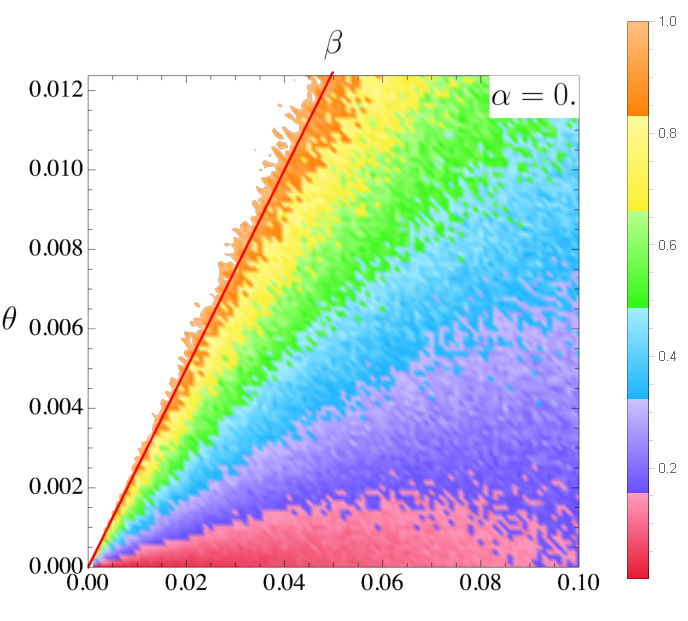
\includegraphics[width=0.45\linewidth]{pdd-gatedep-thres}\quad
    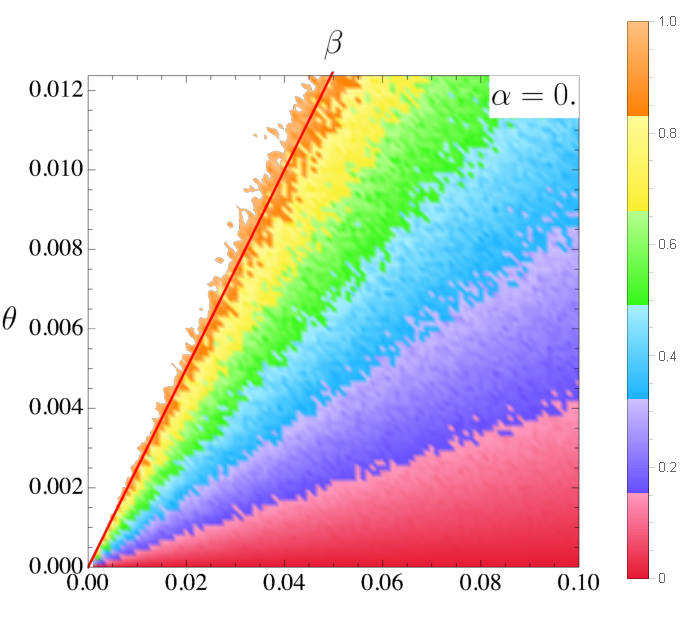
\includegraphics[width=0.45\linewidth]{cdd-gatedep-thres}
    \caption{The noise threshold compared for PDD and $\mathrm{CDD}_3$ simulated at $\alpha=0$.
    The red solid line represents the noise threshold prediction $\eta\le\beta/4$. Different colors represents different levels of noise reduction ration $\beta_\sDD/\beta$ after numerically maximized over random bath operator instances.
    }
    \label{fig:cdd-gatedep-thres}
\end{figure}

In \Figref{fig:cdd-gatedep-thres}, we simulate both PDD and $\mathrm{CDD}_3$ with the gate-dependent noise model. We find that our prediction works pretty well. 


\section{Impact of different measures}
\subsection{Error phase benchmarking}
We reproduce the error phase results in Fig. \ref{fig:pdd-region} in this subsection to make sure that the generation of the Hamiltonian and the usage of the norm are consistent. In Fig. \ref{fig:pdd-region-check-opnorm}(a), The region has similar boundaries as compared In Fig. \ref{fig:pdd-region-check-opnorm}(b) (Fig. \ref{fig:pdd-region})
\begin{figure}
    \centering
    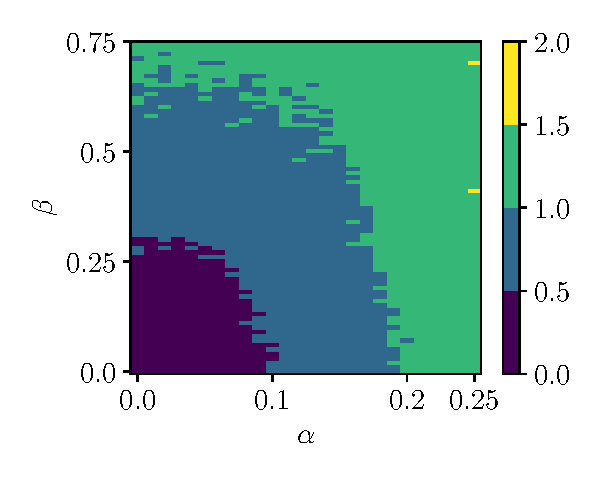
\includegraphics[width=\columnwidth]{error_opnorm}
    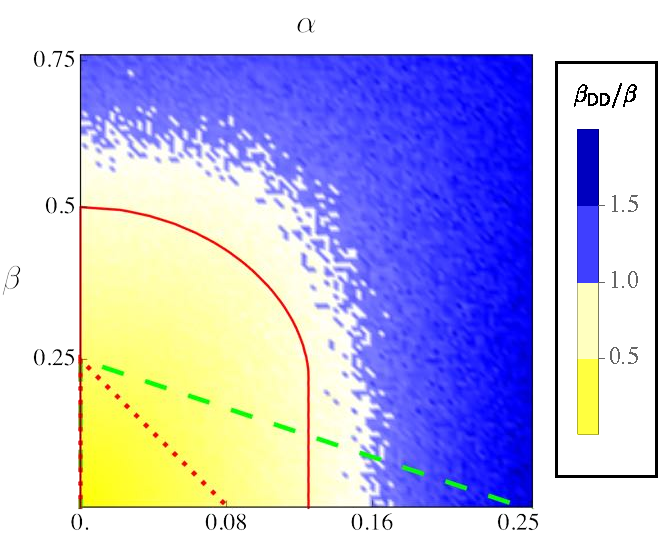
\includegraphics[width=\columnwidth]{pdd-ideal-region}
    \caption{Reproduction of Fig. \ref{fig:pdd-region} by using error phase with operator norm}
    \label{fig:pdd-region-check-opnorm}
\end{figure}

\subsection{Error phase with different norm usage}
Apart from the error phase with operator norm, we also use the Frobenius norm (Hilbert-Schmit norm) to compute the error phase though this is inconsistent with the previous definition. This is to setup possible reference with respect to the channel infidelity measure as $\infid(\cE)\simeq \norm{\Omega_\rSB}_\infty^2$. 

\begin{figure}
    \centering
    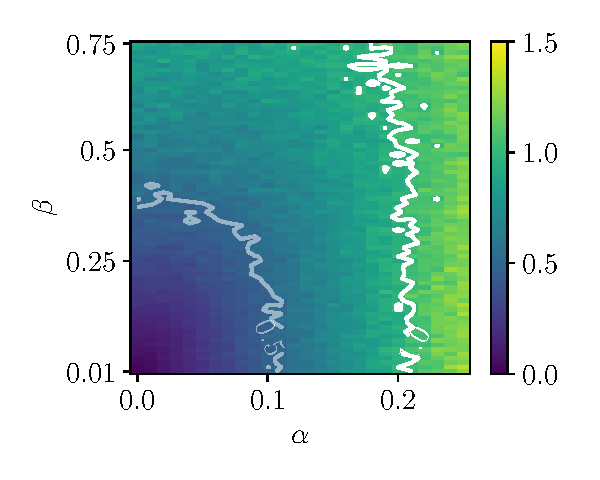
\includegraphics[width=\columnwidth]{error_normhs}
    \caption{Error phase with Hilbert-Schmidt norm} 
    \label{fig:pdd-region-check-norm}
\end{figure}

\subsection{Channel infidelity and trace distance}
We proceed to consider to check channel infidelity as a possible measure whether PDD would work as expected. The detailed implementation is given in Appendix \ref{app:fidelity-numerics}. Note that the definition is given by for a specify channel $\cE$,
\begin{align}
\trdis_{\max}(\cE) &= \max_{\rho\in\cD(\cH)} \tfrac{1}{2} \norm{ (\cI -\cE) (\rho)}_1 \equiv \tfrac{1}{2} \norm{ \cI -\cE}_1, \\
\infid_{\max}(\cE) &\equiv \max_{\rho\in\cD(\cH)} \tr\bigl(\rho\, (\cI -\cE)(\rho)\bigr).
\end{align}
However, for a set of $\alpha$ and $\beta$, there could be various different channels ${\cE}_i$. We have therefore take the maximum over these channels as well thus  
\begin{align}
    \trdis_{\max} &= \max_{{\cE}_i, \rho\in\cD(\cH)} \tfrac{1}{2} \norm{ (\cI - {\cE}_{i}) (\rho)}_1 \equiv \tfrac{1}{2} \norm{ \cI -\cE}_1, \\
    \infid_{\max} &\equiv \max_{ {\cE}_i,\rho\in\cD(\cH)} \tr\bigl(\rho\, (\cI -{\cE}_{i})(\rho)\bigr).
\end{align}
We restrict ourselves to the infidelity of PDD channel and free evolution channel, namely $\infid^{\rm DD}_{\rm max}(\beta, \alpha, \eta)$,  $\infid^{\rm free}_{\rm max}(\beta, \alpha)$. 


We thus consider the ratio of the channel infidelity for DD sequence and that for free evolution, i.e., $\infid^{\rm DD}_{\rm max} / \infid^{\rm free}_{\rm max}$. 

\begin{figure}
    \centering
    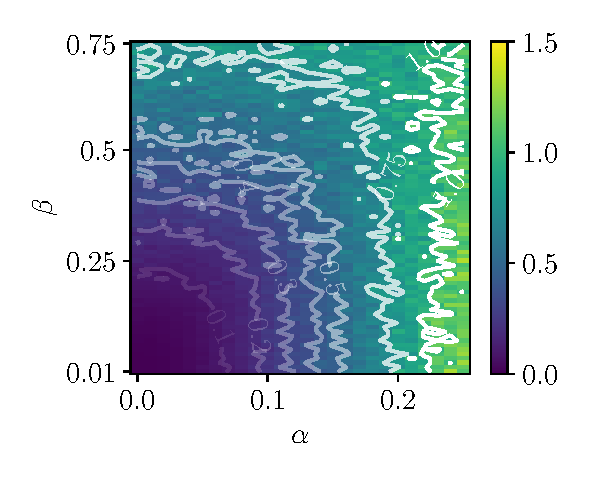
\includegraphics[width=\columnwidth]{infidelity}
    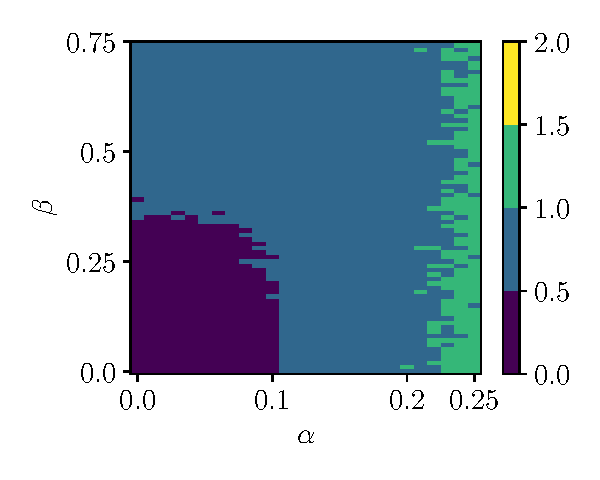
\includegraphics[width=\columnwidth]{infidelity_sqrt}
    \caption{Ratio of $\infid^{\rm DD}_{\rm max} / \infid^{\rm free}_{\rm max}$ and its square root. We consider the ideal situation where the pulses are ideal. For each pair of $\alpha$ and $\beta$, we consider 10000 samples channels ${\cE}_i$} 
    \label{fig:pdd-region-fidelity}
\end{figure}

\begin{figure}
    \centering
    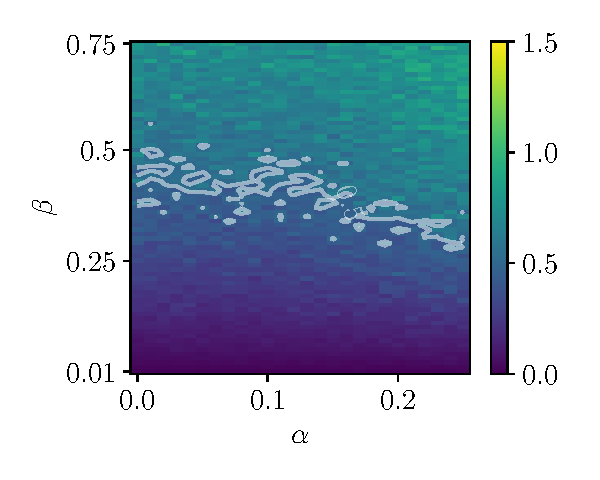
\includegraphics[width=\columnwidth]{trdistance}
    \caption{Ratio of $\trdis^{\rm DD}_{\rm max} / \trdis^{\rm free}_{\rm max}$. We consider the ideal situation where the pulses are ideal. For each pair of $\alpha$ and $\beta$, we consider 10000 samples channels ${\cE}_i$} 
    \label{fig:pdd-region-trdistance}
\end{figure}


\subsection{Difference measures versus $\beta$}
These measures show very different error suppression boundaries. We consider a give measure $\cM$ for DD and free evolution respectively and inspect how it scale with $\beta$. From Fig. \ref{fig:pdd-region-beta}, the error for free evolution (solid lines) are all linear with respect to $\beta$, with different gradients. Channel infidelity for free evolution (blue solid line) is quadratic with respect to $\beta$ which has been proven in Appendix \ref{app:infid-beta-series}. Channel trace distance (orange solid lines), on the other hand, is linearly related to $\beta$. This suggests a different different error tolerance for these measures. For example, free evolution channel trace distance has reached the upper bound defined by Fuchs-van de Graaf inequalities and thus is bounded by the sqrt root of infidelity showing a linear dependence with respect to $\beta$. This would imply a large error for free evolution. On the other hand, the channel trace norm with PDD is quadratic with respect to $\beta$ corresponding to the free evolution infidelity. ({Qns: \color{red} To what extent do they correspond to just a scaling on the parameters?} ). For error phase using operator norm and Frobenius norm, both of them are linear with respect to $\beta$ for free evolutions.

\begin{figure}
    \centering
    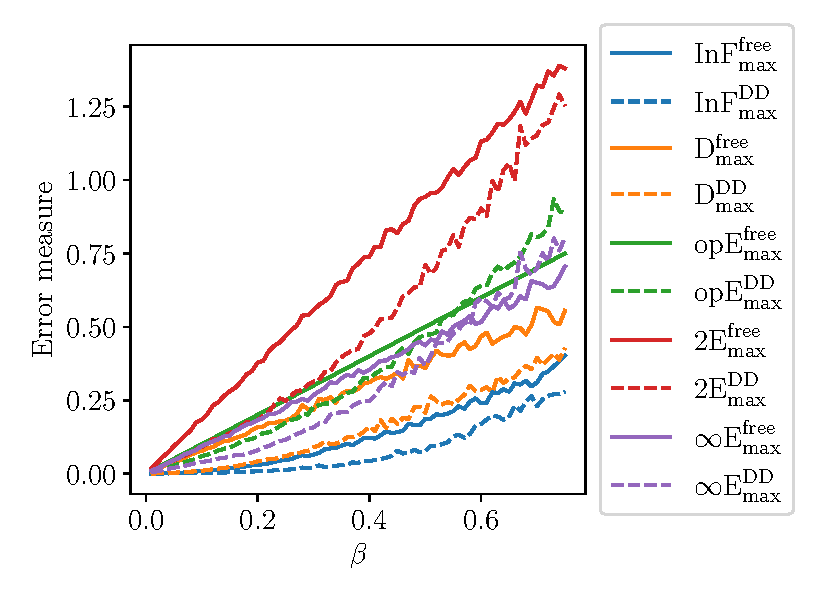
\includegraphics[width=\columnwidth]{error_beta}
    \caption{Different error measures versus $\beta$ at a fix $\alpha$. $\alpha=0.1$. Free evolution with $\Omega$ (solid lines) and evolution under PDD cycle $\Opdd$ (dashed lines) by using channel infidelity (blue), channel trace distance (orange), operator norm (green) (error phase), and Hilbert-Schmidt norm (red).} 
    \label{fig:pdd-region-beta}
\end{figure}




\subsection{Noisy pulse}
\begin{figure*}[ht!]
    \centering
    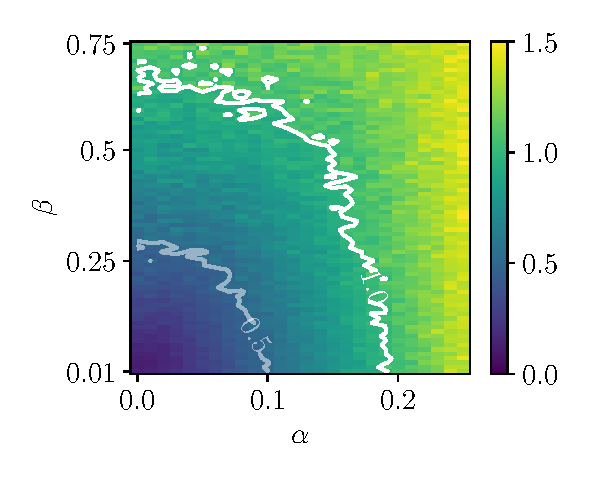
\includegraphics[scale=0.42]{errorphase_eta0.02.pdf}
    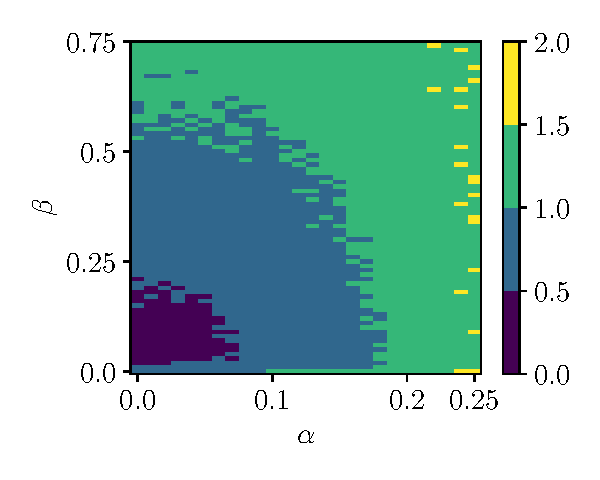
\includegraphics[scale=0.42]{errorphase_eta0.06.pdf}
    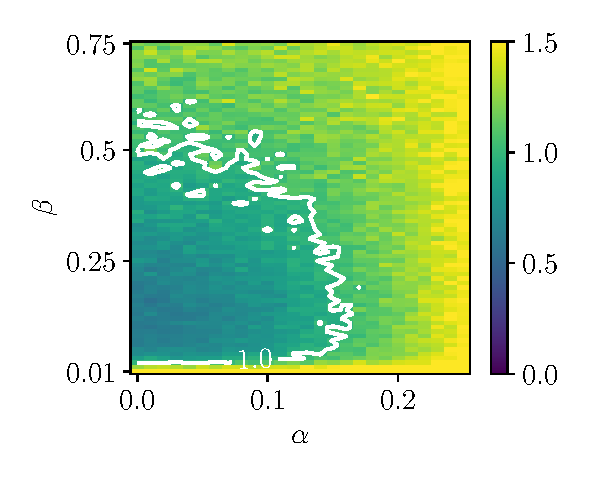
\includegraphics[scale=0.42]{errorphase_eta0.1.pdf}
    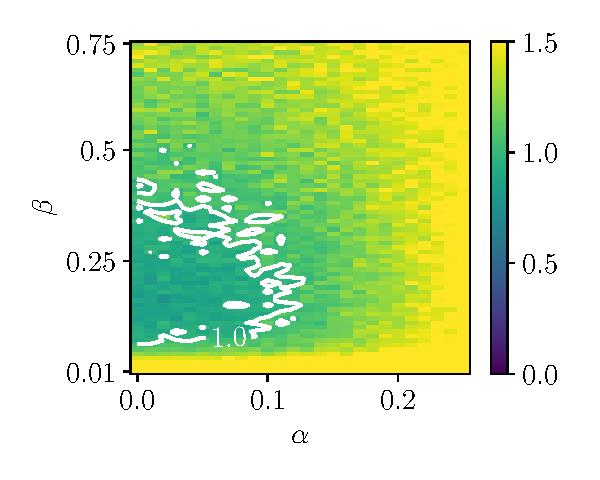
\includegraphics[scale=0.42]{errorphase_eta0.14.pdf}
    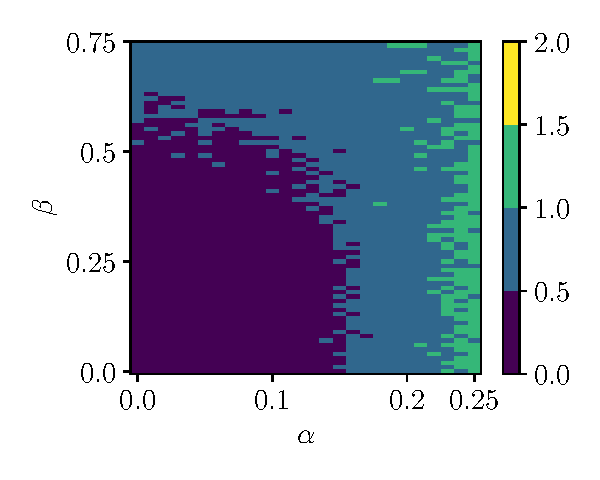
\includegraphics[scale=0.42]{infidelity_eta0.02.pdf}
    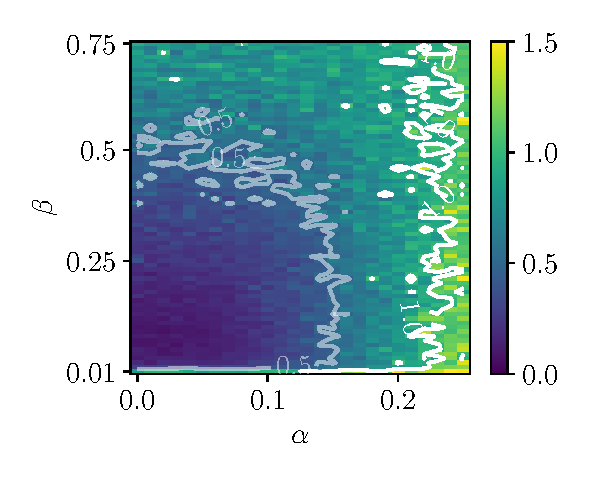
\includegraphics[scale=0.42]{infidelity_eta0.06.pdf}
    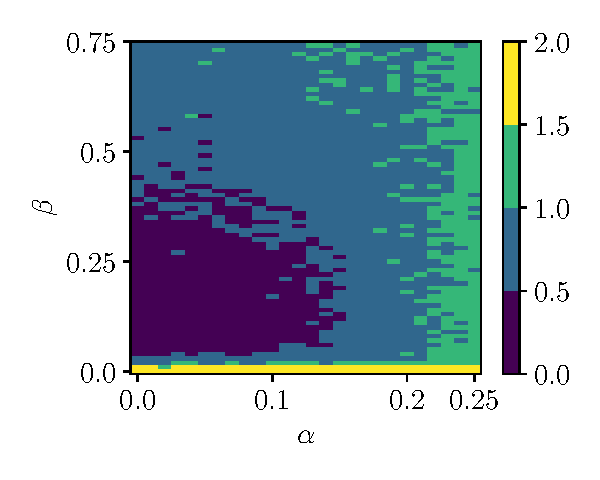
\includegraphics[scale=0.42]{infidelity_eta0.1.pdf}
    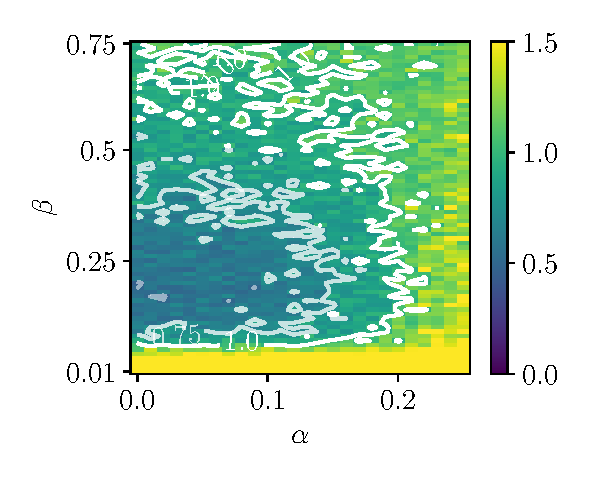
\includegraphics[scale=0.42]{infidelity_eta0.14.pdf}
    \caption{Top panels: reproduction of the error phase results in Fig. \ref{fig:npdd-reg-tho}. Bottom panels: Noise reduction region using channel infidelity. The strength of noise in the pulse $\theta = 0.02,~0.06,~0.1,~0.14$ from left to right. } 
    \label{fig:noisy-pulse-comparison}
\end{figure*}

By using different measures, we do see a different noise reduction region. This is is demonstrated by the comparison between noise suppression region using error phase and channel infidelity in Fig. \ref{fig:noisy-pulse-comparison}. The noise suppression region by channel infidelity is larger than that of the error phase.







\section{conclusion}
The conclusion that CDD is superior to PDD by just looking at \Figref{fig:cdd-noise-removal} should be taken with a grain of salt. 
In general, for CDD,  despite the fact that the
noise decoupling order increases with the concatenation level,
it might not prove helpful for realistic noisy removal purposes. 
From \Figref{fig:cdd-region}, we find that the absolute-convergence region rapidly shrink with the concatenation level. This means that for a system whose $(\alpha,\beta)$ are not \emph{really} small to start with, our analysis may not work anymore with high concatenation levels due to convergence issue. 
If we consider instead the overlapping region between \Figref{fig:cdd-region} and \Figref{fig:cdd-noise-removal}, the
noise removal criteria as determined by \Eqref{eq:CDD-converge} and \Eqref{eq:CDD-noise-removal} become increasingly stringent as the concatenation level increases.  
In general, high-order CDD may not be a good noise suppression choice for quantum computation. To determine the suitable concatenation level, one needs to weigh the costs and benefits between introducing more errors by more pulses and the better noise removal capability promised by of higher order CDD .





\bibliography{references}

\appendix
\section{Channel infidelity series in error phase}\label{app:infid-beta-series}
In the following, we show that the channel infidelity function \Eqref{eq:inf-def} for a CPTP channel does not contain terms linear in the error phase when written as a infinite series.
Alternative, by writing  
$\Omega =  \alpha \Omega_\rB + \beta \Omega_{\rSB}$ for real numbers $\alpha$ and $\beta$, wee need to show that $\infid(\cE|\rho)$ does not contain any term linear in $\beta$.

The equality $\trB \ad_{\Omega_{\rB}} = 0$ from \Eqref{eq:trBad} allows us to freely apply a pure-bath time evolution before $\trB$:
\begin{equation}
    \trB \Ad \upe^{\upi \alpha \Omega_{\rB}} = \trB \upe^{\upi \alpha \ad_{\Omega_{\rB}}} = \trB \upe^{0} = \trB,
\end{equation}
where $\Ad X (\placeholder)\equiv X (\placeholder) X^\dagger$.
Therefore
\begin{equation}\label{eq:rhoS-interaction}
\begin{split}
\cE(\rhoS) &= \trB\, \Ad \upe^{-\upi (\alpha \Omega_{\rB} + \beta \Omega_{\rSB})} \, \rho(0)\\
&= \trB\, \Ad \upe^{\upi \alpha \Omega_{\rB}}\, \Ad \upe^{-\upi (\alpha \Omega_{\rB} + \beta \Omega_{\rSB})} \, \rho(0) \\
&= \trB\, \Ad \upe^{\upi \alpha \Omega_{\rB}} \upe^{-\upi (\alpha \Omega_{\rB} + \beta \Omega_{\rSB})}\, \rho(0).
\end{split}
\end{equation}
We can expand the product of the above exponential functions as a Taylor series of $\beta$:
\begin{align}
\upe^{\upi \alpha \Omega_{\rB}} &\upe^{-\upi (\alpha \Omega_{\rB} + \beta \Omega_{\rSB})} 
= 1 + \beta
\left. \upe^{\upi \alpha \Omega_{\rB}} \frac{d}{d\beta}\upe^{-\upi (\alpha \Omega_{\rB} + \beta \Omega_{\rSB})} \right|_{\beta=0} \notag \\
&+ \frac{\beta^2}{2}
\left. \upe^{\upi \alpha \Omega_{\rB}} \frac{d^2}{d\beta^2}\upe^{-\upi (\alpha \Omega_{\rB} + \beta \Omega_{\rSB})} \right|_{\beta=0} +\cO(\beta^3) \notag \\
={}& 1 - \upi \beta K_1 -\frac{\beta^2}{2} (K_1^2+ \upi K_2)  + \cO(\beta^3),
\end{align}
where we have defined two Hermitian operators,
\begin{align}
& K_1 = \sum_{n=0}^{\infty} \frac{(\upi \alpha)^n}{(n+1)!}\ad^n_{\Omega_{\rB}}(\Omega_{\rSB}), \\
& K_2 = \upi \sum_{n=1}^\infty \frac{(\upi \alpha)^n}{(n+2)!}\sum_{k=1}^n \ad^{n-k}_{\Omega_{\rB}} \ad_{\Omega_{\rSB}} \ad^k_{\Omega_{\rB}} (\Omega_{\rSB})
\end{align}
According to the exponential function derivative  formula:
\begin{equation}
\frac{d}{dt}\upe^{\Omega(t)}=\upe^{\Omega(t)} \sum_{n=0}^\infty \frac{(-1)^n}{(n+1)!}\ad_{\Omega(t)}^n\left(\frac{d}{dt}\Omega(t)\right).
\end{equation} 
Apply the Taylor series to \Eqref{eq:rhoS-interaction} and expand the conjugation, we have
\begin{multline}
\cE(\rhoS) = \rho_\rS - \upi \beta \trB[K_1,\rho(0)] - \upi \frac{\beta^2}{2}\trB[K_2,\rho(0)] \\
- \frac{\beta^2}{2}\trB[K_1,[K_1,\rho(0)]] + \cO(\beta^3).
\end{multline}
Now that the second and third term have the single commutator form, which vanishes after taking trace product with $\rho_\rS$ (see \Eqref{eq:1st-infid}). The smallest term left in the infidelity expression is therefore the $\beta^2$ term with conjugation by $K_1(\alpha)$. Thus 
proves our proposition. 

\section{Norm inequalities}\label{app:norm-ineq}

\section{Leading orders of polynomials}\label{app:polynomials}

To make the idea of ``leading power'' precise, we take the following conventions. 
For a polynomial $\sum_{k} a_k x^k$ with real coefficients, we define its leading power as the smallest number $k$ such that $a_k\neq 0$. For a polynomial with multiple parameters, the leading power is defined as the smallest combined power with nonzero coefficient.
We say $p\mathbin{\sim}q$ if $p$ and $q$ have the same leading power, $p\ll q$ if the leading power of $p$ is greater than $q$, $p\lesssim q$ if the leading power of $p$ is greater or equal to $q$. This establishes a transitive ordering for the polynomials. This notation is consistent with the usual inequalities for nonnegative polynomials (i.e., polynomials with nonnegative output for nonnegative input parameters). If two nonnegative polynomial satisfies $p\le q$ for all nonnegative parameters, then $p\lesssim q$; but the converse cannot be said.
If $p\lesssim q$, then $p+q \sim q$. In general $\sum_i p_i \sim \max_i \{ p_i \}$, where the maximization is defined by $p_i \lesssim \max_i \{ p_i \}, \forall i$ and represents the leading order term of the series $\sum_i p_i$. 

\section{Implementation for channel infidelity and channel trace distance}\label{app:fidelity-numerics}
For a single-qubit system coupled with a bath, we denote the free evolution Hamiltonian for time $\Dt$ as:
\begin{equation}\label{eq:omega-sq}
    \Omega = \Dt H = \sigma_0 \otimes B_0 + \sum_{i=1}^3 \sigma_i \otimes B_i,
\end{equation}
where 
$\{\sigma_i\}$ are the system space Pauli operators and
$\{B_i\}$ are the Hermitian bath operators with $\tr(B_0)=0$. The bath operators $B_i$ can be arbitrary dimensional, but are normalized such that  
\begin{equation}\label{eq:bathops-norm}
\opnorm{\Omega}
=
\begin{pmatrix}
\norm{B_0}\\
\norm[\Big]{\sum_{i=1}^3 \sigma_i \otimes B_i}
\end{pmatrix}\equiv\begin{pmatrix}
    \alpha\\
    \beta
    \end{pmatrix}.
\end{equation}

 

To reduce noise, we perform dynamical decoupling by periodically
applying the pulse cycle ``$-X-Z-X-Z$''.
The is also known as PDD scheme.
This cycle is sometimes referred to the universal decoupling sequence and it can suppress all types of noise on the qubit. 
Under the ideal-pulse assumption, the time evolution operator for the PDD cycle is:
\begin{equation}
Z \upe^{-\upi \Omega} X \upe^{-\upi \Omega} Z \upe^{-\upi \Omega} X \upe^{-\upi \Omega} 
\equiv \upe^{-\upi\Opdd},
\end{equation}
where an effective Hamiltonian $\Opdd$ is defined for the time evolution. When the pulses are imperfect, we model the noisy in the pulses with a noise operator $V(\eta)$ such that the pulses are given by $\tilde{P}_i = P_iV(\eta)$ where $\eta$ is a generic parameter to characterize the noise strength. It follows the time evolution operator for the noisy PDD cycle is given by
\begin{equation}
    \tilde{Z} \upe^{-\upi \Omega} \tilde{X}  \upe^{-\upi \Omega} \tilde{Z} \upe^{-\upi \Omega} \tilde{X} \upe^{-\upi \Omega} 
    \equiv \upe^{-\upi\tilde{\Omega}_{\mathsf{P}}},
\end{equation}
In the following, we consider the unitary noise, often due to over rotation, e.g., $\Pt_i = P_i \upe^{-\upi \vec{\sigma} \cdot\vec{\theta}}$, where $\vec{\theta} = (\theta_1,\theta_2, \theta_3)^\transpose$. In this case, the noise strength parameter $\eta$ is characterized by $\eta\equiv\norm{\vec{\theta}}\equiv\theta$.




The output system state under the free evolution Hamiltonian $\Omega$ and the PDD effective Hamiltonian $\Opdd$ given an arbitrary initial state $\rhoS\in\cH_\rS$ and can be written as
\begin{align}\label{eq:output-rhos}
    \cE_{\Omega}(\rhoS) &= \trB  \left(
\upe^{-\upi \Omega} (\rhoS \otimes \rhoB) \upe^{\upi \Omega} \right), \\
    \cE_{\Opdd}(\rhoS) &= \trB  \left(
\upe^{-\upi \Opdd} (\rhoS \otimes \rhoB) \upe^{\upi \Opdd} \right),
\end{align}
where $\rhoB\in\cH_\rB$ is the initial bath state; $\trB(\placeholder)$ is the partial trace over $\cH_\rB$. Since the noise map $\cE$ is determined by $\Omega$ and $\rhoB$, to evaluate the channel infidelity, we consider the infinite temperature state (maximally mixed state) to be $\rhoB$ and random bath operators $\{B_i\}$ for both $\Omega$ and $\Opdd$.


Given a channel $\cE$, the trace distance and infidelity are given by
\begin{align}\label{eq:trd-def}
    \trdis(\cE|\rho) &\equiv \trdis(\rho, \cE(\rho)) = \tfrac{1}{2} \norm{ (\cI -\cE) (\rho)}_1, \\
    \infid(\cE|\rho) &\equiv 1- \fid(\rho, \cE(\rho)) = \tr\bigl(\rho\, (\cI -\cE)(\rho)\bigr).\label{eq:inf-def}
\end{align}
respectively. To get rid of the state dependence and Hamiltonian dependence (due to random bath operators) , we consider a maximization of the trace distance and infidelity over all the pure input state and random bath operators,
\begin{align}
    \trdis_{\max} &= \max_{{\cE}, \rho\in\cD(\cH)} \tfrac{1}{2} \norm{ (\cI - {\cE}) (\rho)}_1 \equiv \tfrac{1}{2} \norm{ \cI -\cE}_1, \\
    \infid_{\max} &\equiv \max_{ {\cE},\rho\in\cD(\cH)} \tr\bigl(\rho\, (\cI -{\cE})(\rho)\bigr).
\end{align}
We restrict ourselves to the infidelity of PDD channel and free evolution channel, namely $\infid^{\rm DD}_{\rm max}(\beta, \alpha, \eta)$,  $\infid^{\rm free}_{\rm max}(\beta, \alpha)$. 

In the figures, we thus consider the ratio of the channel infidelity and channel trace distance for DD sequence and that for free evolution, i.e., $\infid^{\rm DD}_{\rm max} / \infid^{\rm free}_{\rm max}$ and $\trdis^{\rm DD}_{\rm max} / \trdis^{\rm free}_{\rm max}$, respectively. The maximization is done over 10000 samples for different initials states and random bath operators with a fixed bath density matrix given by the infinite temperature state (maximally mixed state).  



\end{document}
